%!TEX root = ../thesis.tex
%!TEX TS-program = lualatex
% vim:fenc=utf-8
% vim:fdm=marker



% preambulo latex 
\documentclass[11pt]{article}
\usepackage[spanish,es-lcroman,es-nodecimaldot]{babel}
\usepackage{amsmath,amsfonts,amssymb,units,xcolor}
\usepackage{graphicx,tabularx}
\usepackage{booktabs}
\usepackage{multirow}
\usepackage{fancyhdr}
\usepackage{listings}
\usepackage{hyperref}
\usepackage{blindtext}
\usepackage{lastpage}
\usepackage{fontspec}
\usepackage{titletoc}
\usepackage{titlesec}
\usepackage[export]{adjustbox}
\usepackage[letterpaper,left=3cm,right=2cm,top=2cm,bottom=2cm]{geometry}
\usepackage[sort&compress,authoryear]{natbib}
\usepackage[justification=centerlast,labelfont=bf,font=scriptsize,
            margin=1.5cm,labelsep=period]{caption}


% definir variables
% -----------------
%\newcommand{\boc}{BOC1-LAG}


% configuracion de los paquetes
% -----------------------------

% nueva pagina en cada seccion y subseccion
%\newcommand{\sectionbreak}{\clearpage}
%\newcommand{\subsectionbreak}{\clearpage}
\renewcommand{\contentsname}{Tabla de contenido}

% configuracion de la fuente
\DeclareTextFontCommand{\emph}{\slshape}
\renewcommand\familydefault{\sfdefault}

% marcados de los items en las listas
%\renewcommand{\labelitemi}{$\bullet$}

% espaciado de las lineas para las págines iniciales
\renewcommand{\baselinestretch}{1.25} 
\setlength{\parindent}{0mm}
\setlength{\parskip}{2.5mm}

% hipervinculos
\hypersetup{%
    colorlinks,
    linkcolor={red!50!black},
    citecolor={blue!50!black},
    urlcolor={blue!80!black}
    }

% encabezado
\pagestyle{fancy}
\lhead{
\includegraphics[height=0.75cm,valign=c]{./logo_cicese.jpg}\vspace{1pt}}
\chead{}
\rhead{Pág. \thepage/\pageref{LastPage}}
\lfoot{Reporte técnico}
\cfoot{\today{} - Rev 2.0}
\rfoot{CICESE}
\renewcommand{\footrulewidth}{0.4pt}

% pagina de titulo
\title{
  \vspace{2em}
  \Large{\bfseries Reporte Técnico} \\
  \vspace{3em}
  \LARGE{\bfseries Corrección de la elevación de la superficie libre y la
  velocidad del viento debido el movimiento de la BOMM} \\
  \vspace{3em}
}
%
\author{
  
\includegraphics[height=2cm,valign=c]{./logo_cicese.jpg} \\
  \vspace{0.5ex} \\
  Grupo de oleaje \\
  \small{Departamento de Oceanografía Física} \\
  \small{Centro de Investigación Científica y de Educación Superior} \\
  \small{Ensenada, B.C., México} \\
  \vspace{2em} \\
}
\date{
  \today \\
  Elaboró: D.S.P. Zapata \\
  Revisión 2.0
  \vspace{2em} \\
  \begin{figure}
    \centering
    
\includegraphics[height=2.1cm,valign=c]{./logo_cigom.jpeg}
    \hspace{0.5cm}
    
\includegraphics[height=2.3cm,valign=c]{./logo_sener.jpg}
  \end{figure}
  \vfill
}


%  empezar documento    
% =============================================================================
\begin{document}

% crear titulo
\maketitle
\thispagestyle{empty}
\newpage
\thispagestyle{fancy}
\tableofcontents
\newpage


% introduccion {{{
\section{Introducción}

En este reporte se presenta el procedimiento y la metodología que se siguió para
aplicar la corrección de los datos observados por el anemómetro sónico y el
arreglo de alambres de capacitancia, debido a los movimientos inerciales de la
boya. En primer lugar se presenta la metodología para obtener los ángulos que
definen la posición y la orientación de la boya a partir de las mediciones de
los giroscopios y los acelerómetros. La BOMM (Boya Oceanográfica y de
Meteorología Marina) cuenta con un IMU (\emph{Inertial Motion Unit}) SBS
Ekinox2-M el cual tiene tres acelerómetros y tres giroscopios.  Adicionalmente,
la orientación de la boya se puede obtener de dos maneras, una es usando el
magnetómetro que viene incorporado en el Signature y otra es mediante una
estimación indirecta a partir de la dirección del viento que se obtiene de la
estación meteorológica Gill Maximet GMX-600. Para una completa descripción de
las características de la boya ver la ficha técnica (BOMM1-ITS).

% }}}

% definicion del marco de referencia {{{
\section{Definición marco de referencia}

El marco de referencia que usa el Ekinox2-M es un sistema de ``mano derecha''
con el eje $x$ positivo apuntando en la dirección de sujeción de la boya, el
eje $y$ positivo a $90^\circ$ en sentido horario del eje $x$ y el eje $z$
positivo apuntando hacia abajo, es decir, hacia el fondo del mar
(Fig.~\ref{fig:ekinox_reference_frame}).

\begin{figure}[htpb]
  \centering
  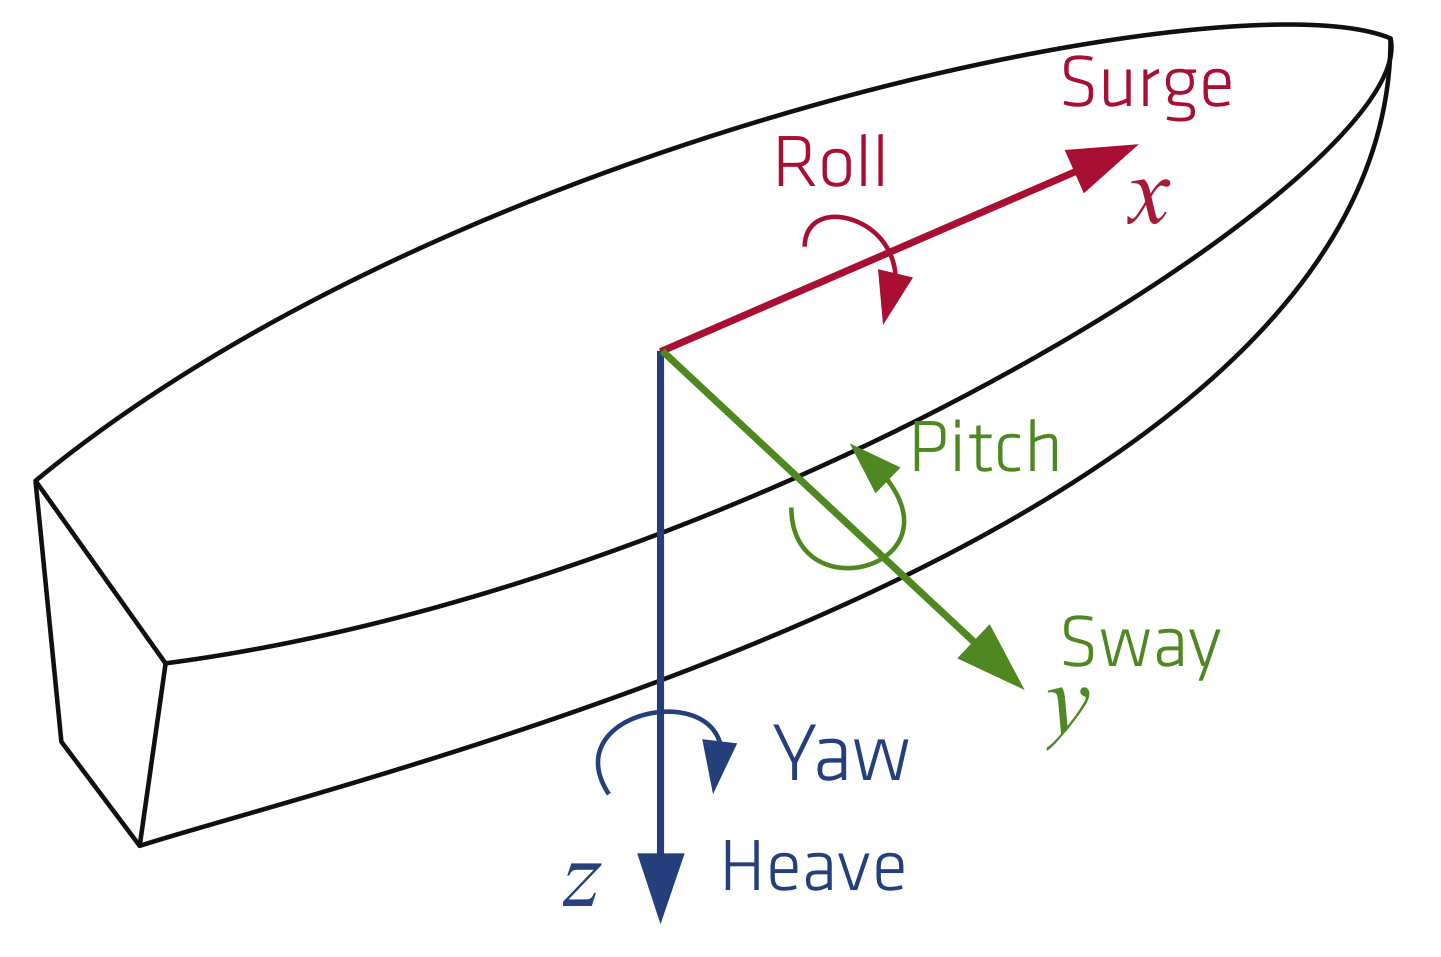
\includegraphics[width=0.6\linewidth]{./figures/ekinox_reference_frame.png}
  \caption{
    Marco de referencia del IMU en el que se muestran la convención que se sigue
    para definir el sentido del movimiento y los ángulos de orientación e
    inclinación de la boya.
  }
  \label{fig:ekinox_reference_frame}
\end{figure}

En español no hay una manera generalizada y comúnmente aceptada de definir los
movimientos y los ángulos, por lo que para los fines de este trabajo se usarán
los términos en inglés. Sin embargo, se evitará el abuso de estos términos en
inglés, dando su definición cuando sea posible. Los movimientos lineales que
sufre la boya, en el marco de referencia de la
Fig.~\ref{fig:ekinox_reference_frame} son:

\begin{description}
  \item[Surge] Movimiento horizontal a lo largo del eje $x$.
  \item[Sway] Movimiento horizontal transversal al eje $x$.
  \item[Heave] Movimiento de ascenso y descenso, es decir,
    a lo largo del eje $z$.
\end{description}

De la misma manera, los ángulos que definen la inclinación y la orientación de
la boya son:

\begin{description}
  \item[Roll] Movimiento de rotación alrededor del eje $x$.  Se entiende como
    una inclinación lateral de la boya. Se denota por la letra griega $\phi$.
  %
  \item[Pitch] Movimiento de rotación alrededor del eje $y$. Se entienda como
    una inclinación frontal de la boya. Se denota por la letra griega $\theta$.
  %
  \item[Yaw] Movimiento de rotación alrededor del eje $z$. Se denota por la
    letra griega $\psi$ y está definido entre $0$ y $2\pi$ y su punto de
    referencia es el norte geográfico. Se entiende como la orientación del norte
    de la boya.
\end{description}

% cambio de marco de referencia {{{
\subsection{Cambio de marco de referencia}
\label{sub:cambio_de_marco_de_referencia}

Debido a que el IMU se encuentra montado sobre una plataforma móvil, es decir,
la boya, todas las mediciones vectoriales que se realicen se deben referenciar a
un marco de referencia inercial. Por ejemplo, la boya registra la elevación de
la superficie libre por medio de alambres de capacitancia, pero como la boya se
mueve con el oleaje, los datos de los alambres deben ser corregidos para
ponerlos en un sistema de referencia que no se esté moviendo con la boya. Lo
mismo sucede con el anemómetro sónico que registra la velocidad del viento, pero
debido a los movimientos de la boya, aparecen velocidades espúreas que se
remueven al cambiar el marco de referencia por uno referido a tierra.

Existen varias maneras de representar la rotación de un vector alrededor de un
vector unitario, por ejemplo, los ángulos de Euler, los cuaterniones y la
representación ángulo-eje. En este caso se usa la matriz de rotación, que aunque
no es la más eficiente computacionalmente, es la más fácil de visualizar. La
matriz de rotación está definida por tres vectores unitarios que definen el
sistema de coordenadas. Esta matriz transforma del sistema coordenado de la
boya, representado por la letra $B$ de \emph{body} al sistema inercial, denotado
con la letra $E$ de \emph{earth}. La matriz de rotación es la combinación de
tres matrices, que representan la rotación alrededor de cada uno de los ejes
coordenados. Existen diversas combinaciones que dan formas diferentes de la
matriz de rotación, en este caso se usó la conveción aeronáutica o $zyx$, en la
cual el orden de las rotaciones está dado por:

\begin{equation}
  \mathbf{R} = \mathbf{R}_z(\psi) \mathbf{R}_y(\theta) \mathbf{R}_x(\phi),
\end{equation}
%
\begin{equation}
  \mathbf{R} =
  \left[
    \begin{array}{c c c}
      \cos{\psi} & -\sin{\psi} & 0 \\
      \sin{\psi} &  \cos{\psi} & 0 \\
      0          & 0           & 1
    \end{array}
  \right]
  %
  \left[
    \begin{array}{c c c}
      \cos{\theta}  & 0 & \sin{\theta} \\
      0             & 1 & 0            \\
      -\sin{\theta} & 0 & \cos{\theta}
    \end{array}
  \right]
  %
  \left[
    \begin{array}{c c c}
      1 & 0 & 0 \\
      0 & \cos{\phi} & -\sin{\phi} \\
      0 & \sin{\phi} &  \cos{\phi} \\
    \end{array}
  \right],
\end{equation}
%
\begin{equation}
  \mathbf{R} = \left[
    \begin{array}{c c c}
      %
      \cos{\theta}\cos{\psi} &
      \sin{\phi}\sin{\theta}\cos{\psi} - \cos{\phi}\sin{\psi} &
      \cos{\phi}\sin{\theta}\cos{\psi} + \sin{\phi}\sin{\psi} \\
      %
      \cos{\theta}\sin{\psi} &
      \sin{\phi}\sin{\theta}\sin{\psi} + \cos{\phi}\cos{\psi} &
      \cos{\phi}\sin{\theta}\sin{\psi} - \sin{\phi}\cos{\psi} \\
      %
      -\sin{\theta} &
      \sin{\phi}\cos{\theta} &
      \cos{\phi}\cos{\theta} \\
      %
    \end{array}
  \right].
  \label{eq:rotation_matrix}
\end{equation}

Para transformar un vector que se encuentra en el marco de referencia que se
mueve con la boya, $\mathbf{u}_\mathrm{B}$, al marco de referencia fijo en
tierra, $\mathbf{u}_\mathrm{E}$, dado por la tupla de ángulos de Euler
$\mathrm{T} = (\phi, \; \theta, \; \psi)$, se usa la siguiente ecuación:

\begin{equation}
  \mathbf{u}_\mathrm{E} = \mathbf{R} \cdot \mathbf{u}_\mathrm{B}.
\end{equation}


%}}}


% }}}


% calculo de los ángulos {{{
\section{Inclinación, orientación y movimientos lineales}

En esta sección se presenta el procedimiento que se siguió para el cálculo de
los ángulos que definen la inclinación de la boya (roll y pitch, según la
Fig.~\ref{fig:ekinox_reference_frame}), a partir de la información del IMU
Ekinox2-M.


% Inclinacion de la boya {{{
\subsection{Inclinación de la boya}

Es un problema común en robótica el cálculo de los ángulos de Euler a partir de
un IMU. Los giroscopios miden la tasa de cambio del ángulo en el tiempo, la cual
se debe integrar para obtener una estimación del ángulo. El problema con los
giroscopios es que se presenta una acumulación del error en el tiempo debido a
que no se conocen las condiciones iniciales de la integración. En la
Fig.~\ref{fig:gyroscope_issues} se presentan 30 minutos de datos del ángulo de
inclinación lateral (roll) medido por el Ekinox2-M. Para obtener este ángulo se
usa el método de diferencias finitas hacia atrás y se despeja el valor del
ángulo $\phi_i$ en función del cambio local del mismo $\dot{\phi}_i$ y del paso
de tiempo $\Delta t$, es decir,

\begin{equation}
  \phi_i = \phi_{i-1} + \dot{\phi}_i \Delta t.
\end{equation}

Como se observa en la Fig.~\ref{fig:gyroscope_issues} (línea roja), esta forma
de integrar introduce una tendencia lineal que se conoce como deriva y que es
producto de la acumulación del error en el tiempo. Una forma de solucionar esto,
es removimiento la tendencia lineal a los datos (línea verde). Esto,
evidentemente, introduce un nuevo problema, que es la pérdida de información en
la baja frecuencia, es decir, ya no se conoce el ángulo promedio.  En resumen,
el giroscopio es muy bueno para obtener la variabilidad de las oscilaciones de
de los ángulos de inclinación, pero con él no se puede conocer los valores a
largo plazo.

\begin{figure}[htpb]
  \centering
  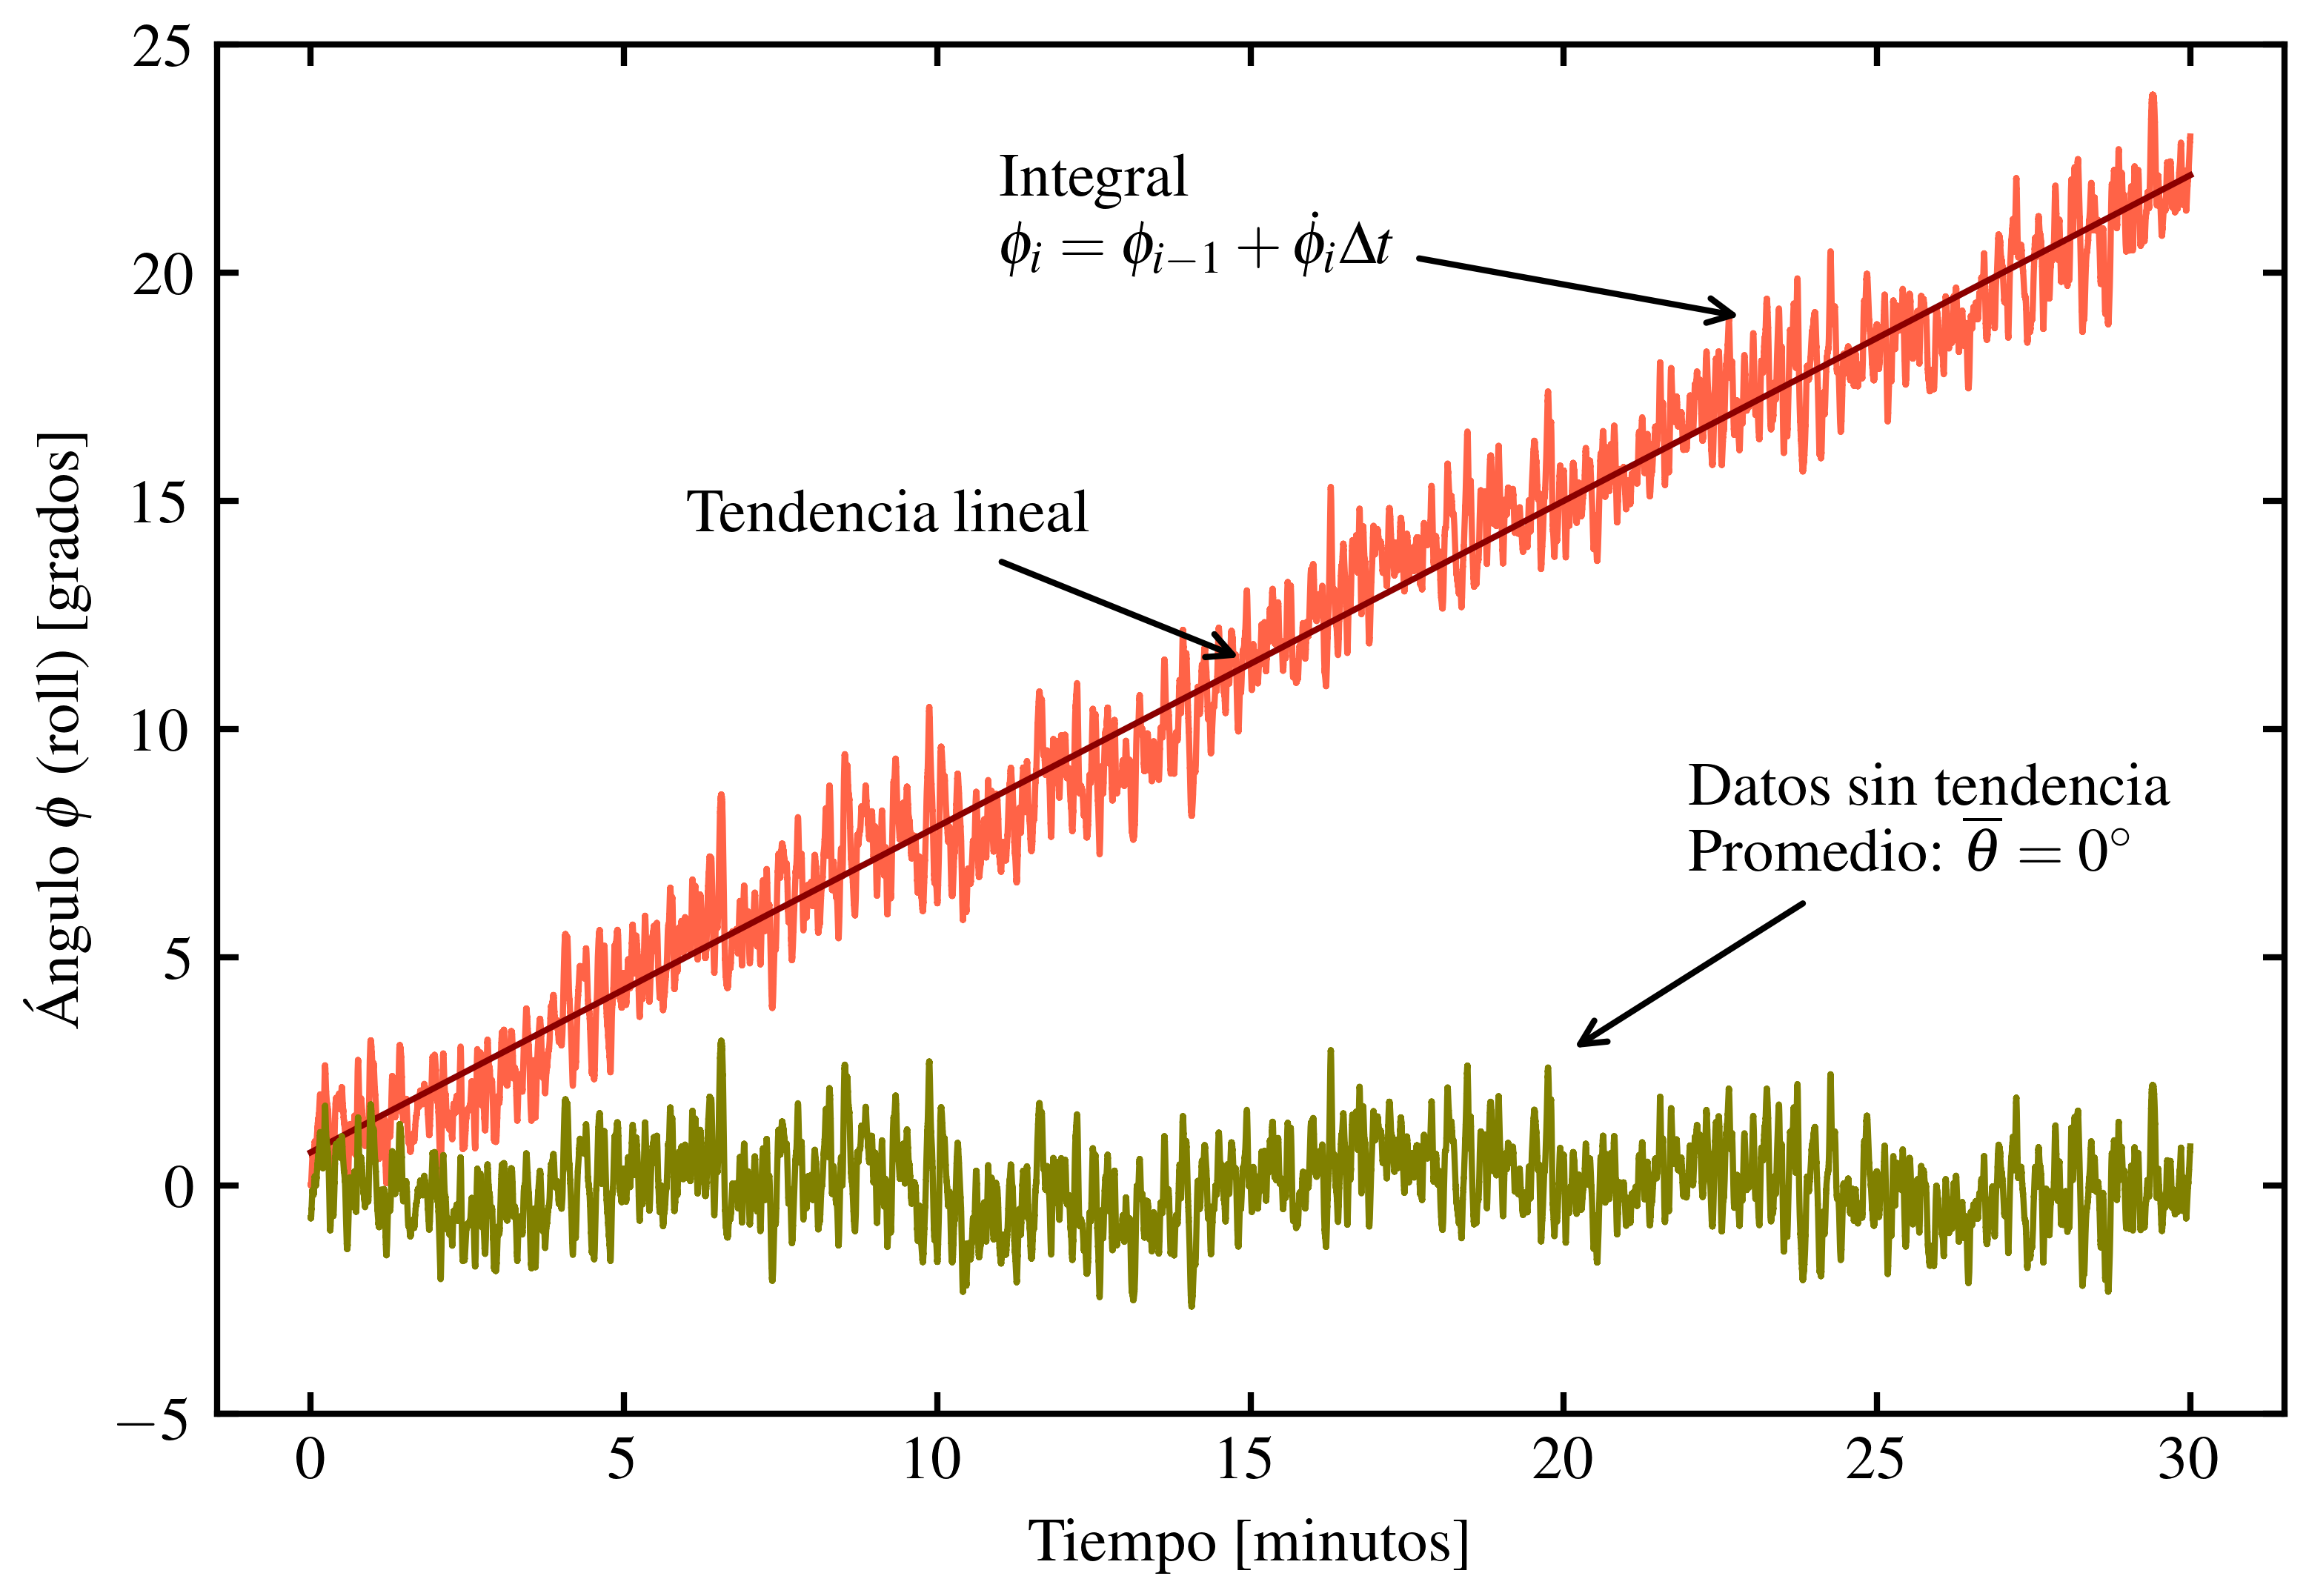
\includegraphics[width=0.8\linewidth]{./figures/gyroscope_issues.png}
  \caption{
    Cálculo de la inclinación de la boya durante un período de medición del
    Ekinox2-M de 30 minutos.
  }
  \label{fig:gyroscope_issues}
\end{figure}

Los acelerómetros, además de ser usados para obtener el cambio de la velocidad
en el tiempo, se pueden usar también para obtener la inclinación de un objeto.
Como el acelerómetro mide todas las fuerzas que están actuando sobre el objeto,
incluyendo la fuerza de la gravedad, se puede usar la matriz de rotación de la
ecuación \eqref{eq:rotation_matrix} para convertir el vector de aceleración que
mide el IMU en el marco de referencia de la boya, al marco de referencia fijo en
tierra, es decir, $\mathbf{g} = \mathbf{R}\cdot\mathbf{a}$. En marco de
referencia inercial, la aceleración de la gravedad solo tiene una componente
vertical, por lo tanto:

\begin{equation}
  %
  \left[
    \begin{array}{c}
      0 \\ 0 \\ g
    \end{array}
  \right] = \mathbf{R} \cdot
  %
  \left[
    \begin{array}{c}
      a_x \\ a_y \\ a_z
    \end{array}
  \right].
  %
\end{equation}

Como en este caso, la inclinación de la boya dada por los ángulos $\phi$ y
$\theta$, es independiente de la orientación, entonces se puede suponer, sin
pérdida de generalidad, que $\psi=0$, haciendo esto, se obtiene la siguiente
matriz de rotación reducida:

\begin{equation}
  %
  \left[
    \begin{array}{c}
      0 \\ 0 \\ g
    \end{array}
  \right] =
  %
  \left[
    \begin{array}{c c c}
      %
      \cos{\theta}  & \sin{\phi}\sin{\theta} &  \cos{\phi}\sin{\theta} \\
      0             & \cos{\phi}             & -\sin{\phi}             \\
      -\sin{\theta} & 0                      & \cos{\phi}\cos{\theta}  \\
      %
    \end{array}
  \right] \cdot
  %
  \left[
    \begin{array}{c}
      a_x \\ a_y \\ a_z
    \end{array}
  \right].
\end{equation}

Con lo cual, resolviendo el sistema de ecuaciones para encontrar las variables
de interés, se tiene que las inclinaciones lateral y frontal de la boya, en
función de las variables del acelerómetro, están dadas por:

\begin{equation}
  \phi = \mathrm{tan^{-1}} \left( \frac{a_y}{a_z} \right),
\end{equation}

y,

\begin{equation}
  \theta = \mathrm{tan^{-1}} \left( \frac{-a_x}{a_y \sin\phi + a_z \cos\phi}
  \right),
\end{equation}

respectivamente.


De nuevo, como los acelerómetros miden todas las fuerzas que se ejercen sobre el
objeto, inclusive las más pequeñas perturbaciones van a generar una gran
cantidad de ruido en la señal calculada. Por tal motivo, la forma de calcular
los ángulos a parir de los acelerómetro requiere que la boya está cercana al
reposo, lo cual no sucede en este caso. Esto quiere decir que los acelerómetros
son útiles para obtener una estimación del ángulo a largo plazo, pero no en el
corto plazo. Por lo tanto se requiere un filtro que deje pasar la información en
en las bajas frecuencias y retenga el ruido de las altas frecuencias.

\begin{figure}[htpb]
  \centering
  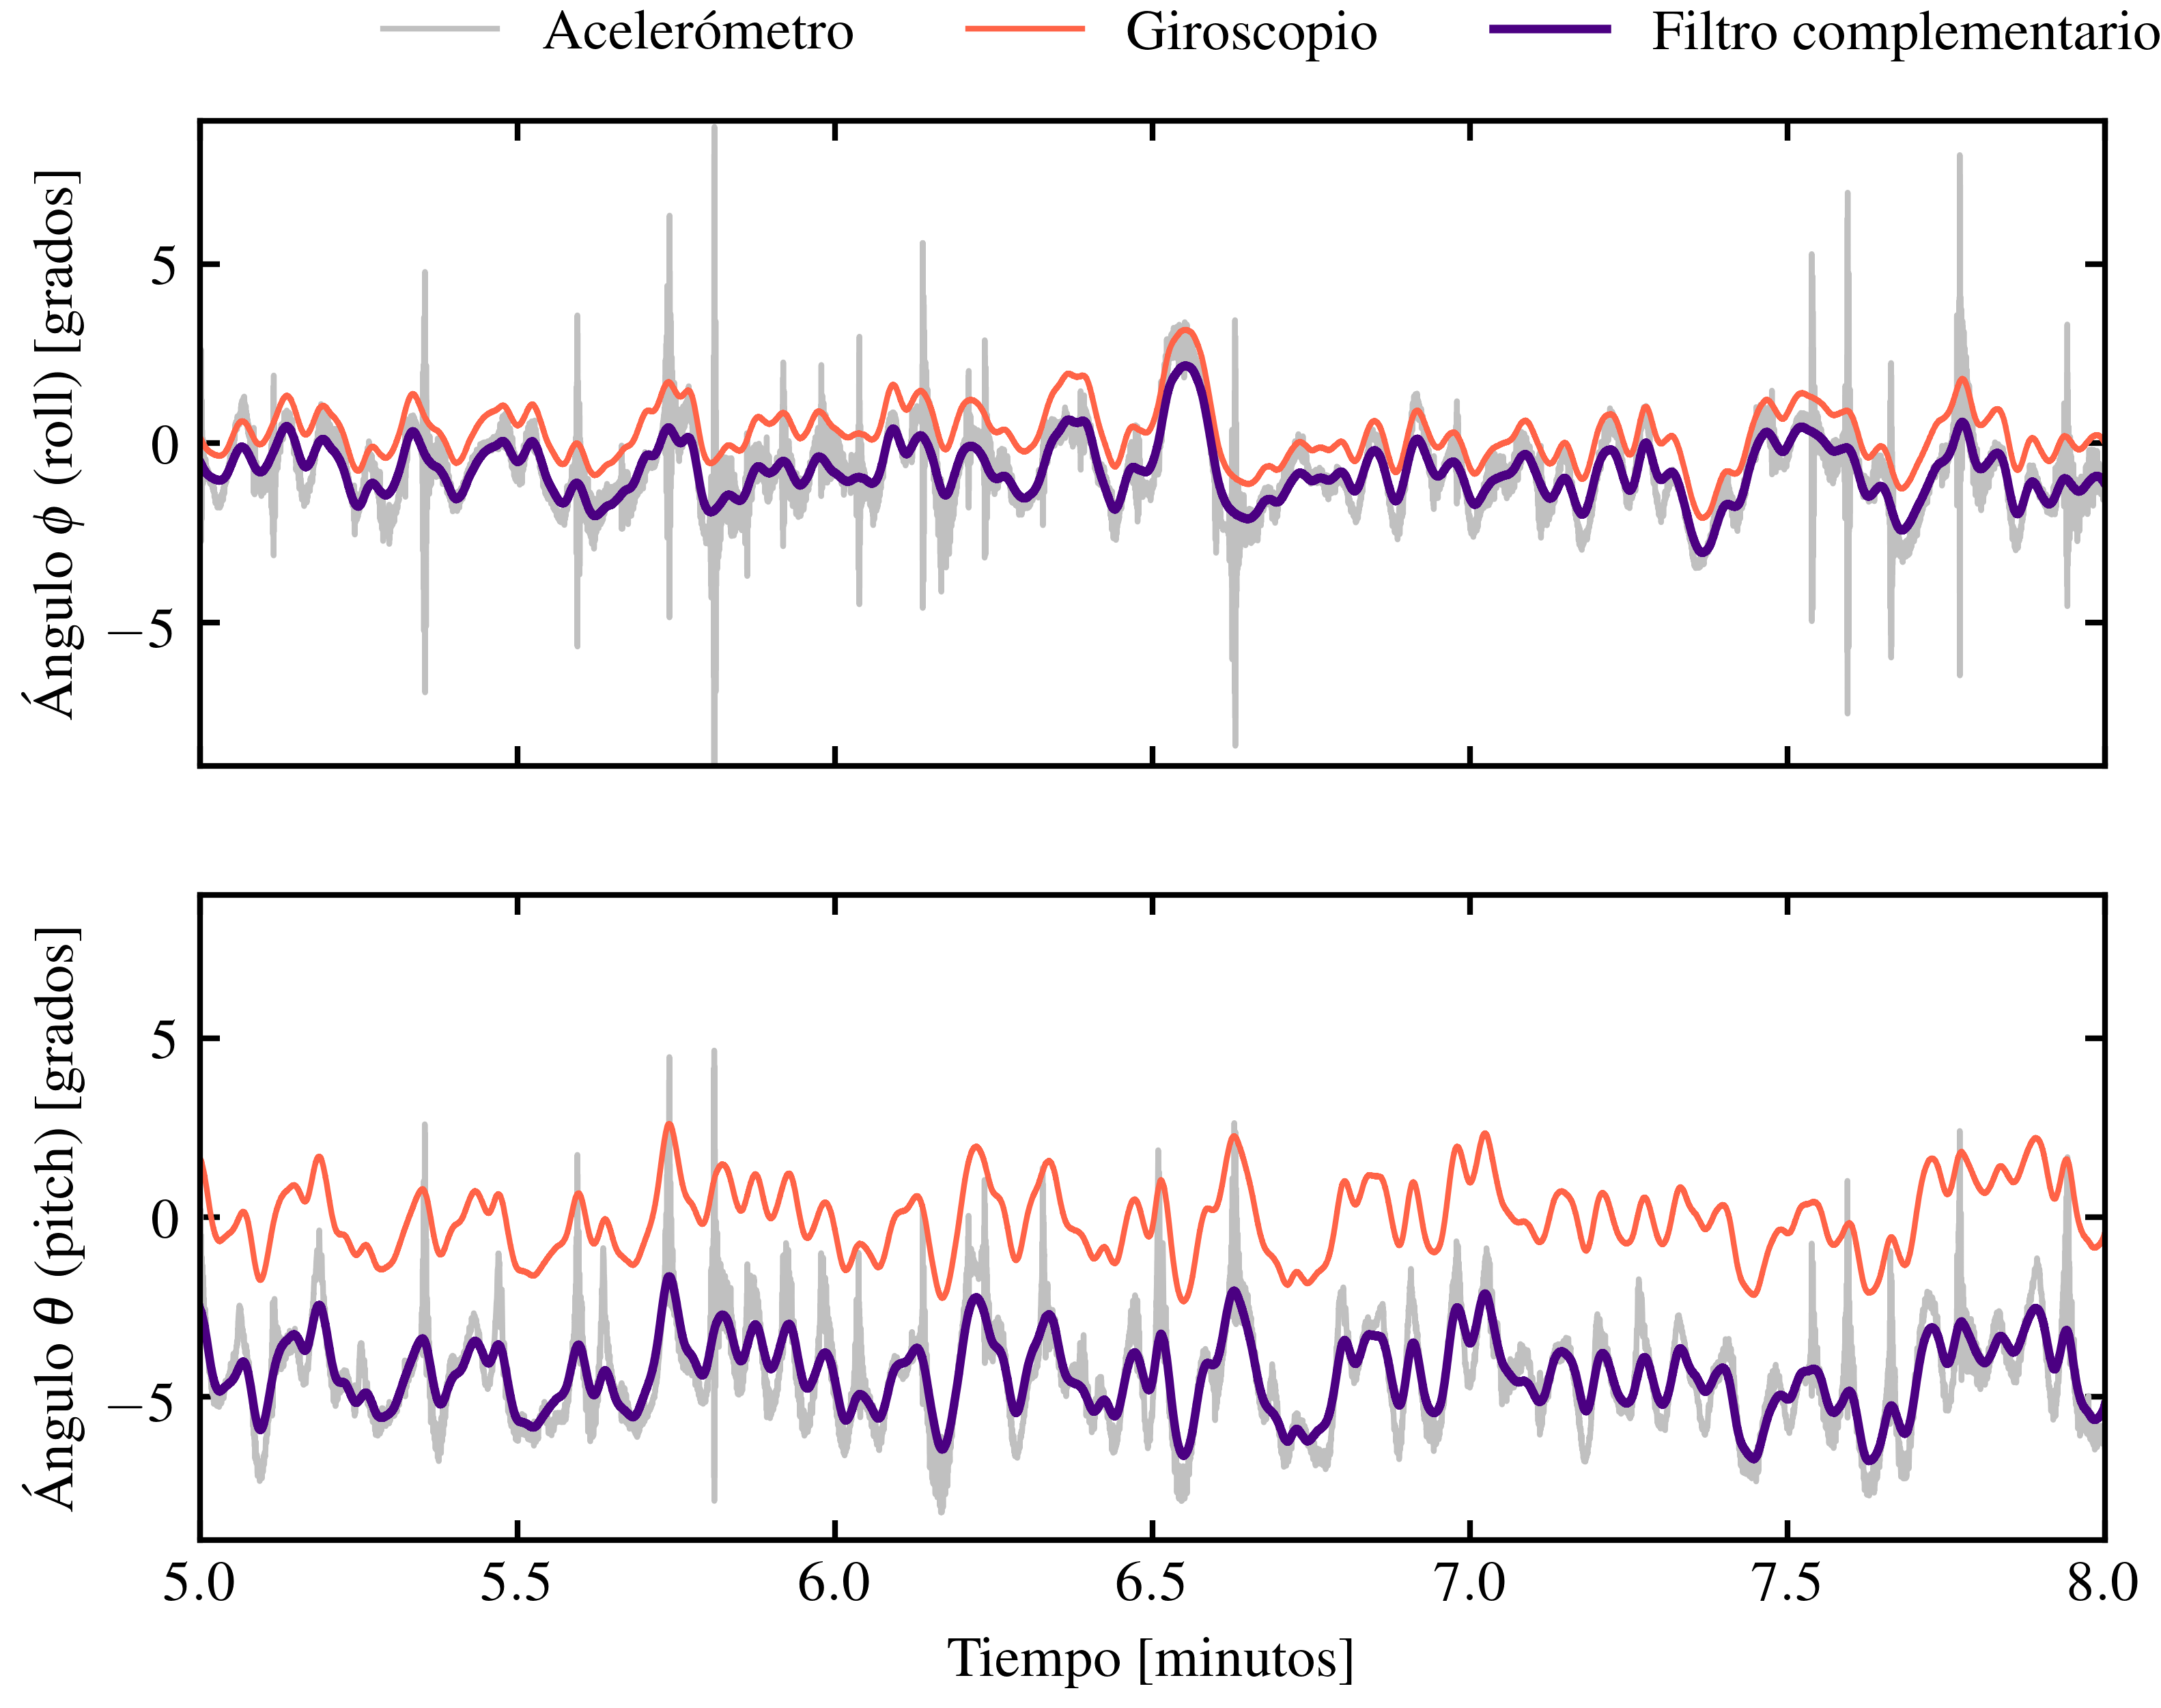
\includegraphics[width=0.8\linewidth]{./figures/gyroscope_vs_accelerometer.png}
  \caption{Estimación de la inclinación mediante un filtro complementario.}
  \label{fig:gyroscope_vs_accelerometer}
\end{figure}

En resumen, el giroscopio da buenos resultados en las altas frecuencias, pero no
``ve'' las bajas frecuencias, mientras que el acelerómetro es útil en las bajas
frecuencias pero presenta una gran cantidad de ruido en las altas frecuencias.
La solución es fusionar las dos señales mediante un filtro complementario, el
cual, está dado por:

\begin{equation}
  \phi_{i} = \alpha \left[\phi_{i-1} + \dot{\phi_{i}} \Delta t \right] +
  (1-\alpha) \phi^\mathrm{acc}_{i}.
\end{equation}

Este filtro corrige la estimación hecha por el giroscopio con el cálculo del
ángulo hecho por el acelerómetro. En otras palabras, el filtro funciona como un
filtro pasa bajas para el acelerómetro y un filtro pasa altas para el
giroscopio. El valor del coeficiente $\alpha$ está relacionado con la frecuencia
de muestreo y la frecuencia de corte, la cual define el intervalo del tiempo que
se considera cómo válido para las mediciones del giroscopio. Por ejemplo, si se
considera que los datos del giroscopio son válidos durante un período de 25
segundos, entonces la frecuencia de corte del filtro complementario será de $f_c
= 1/25\;\mathrm{Hz}$, y se puede demostrar que el valor del coeficiente es
$\alpha = 0.9996$.

Esta forma de implementar el filtro es útil con los datos en tiempo real, pero
es ineficiente cuando se tiene los datos almacenados en un disco, ya que se
requiere una iteración en cada paso de tiempo. De forma práctica, el filtro
complementario se implementó como un filtro digital de butterworth de orden 2,
es decir, el ángulo se calculó como, $\phi(t) = \mathcal{B^*} \left\{
\phi^\mathrm{gyr} \right\} + \mathcal{B} \left\{ \phi^\mathrm{acc} \right\}$,
donde $\mathcal{B}$ representa el operador del filtro pasa bajas que se aplica
sobre los datos del acelerómetro y $\mathcal{B*}$ el operador del filtro pasa
altas que se aplica sobre los datos del giroscopio, ambos para la misma
frecuencia de corte de $f_c$.

En la Fig.~\ref{fig:gyroscope_vs_accelerometer} se presenta un ejemplo de la
estimación de los ángulos de inclinación lateral (arriba) y frontal (abajo),
tanto del acelerómetro (línea gris) como del giroscopio (línea verde). Se
muestra también la estimación de los ángulos con el filtro complementario (línea
azul). Se observa la estimación del giroscopio está centrada en cero, por lo que
no tiene información sobre el ángulo promedio, a pesar de esto la variabilidad
está bien representada. Por otro lado, la estimación del acelerómetro, presenta
una cantidad exagerada de ruido, pero a su vez, estima muy bien el valor
promedio del ángulo en intervalos de tiempo pequeños. Finalmente, la señal que
se obtiene al aplicar el filtro complementario combina las dos señales
anteriores para obtener una mejor estimación de los ángulo.

Con el espectro en frecuencia se puede comprobar cuáles son las frecuencias que
deja pasar el filtro y cuáles son las que retiene. En la
Fig.~\ref{fig:spectra_pitch_and_roll} se presentan los espectros que
corresponden a los dos ángulos calculados de las tres formas. Se observa que la
estimación que se hace con el acelerómetro (línea gris), presenta una gran
cantidad de ruido en las altas frecuencias. Por otro lado, se observa que el
filtro complementario (línea azul) toma los valores del giroscopio en las altas
frecuencias y los del acelerómetro en las bajas frecuencias.

\begin{figure}[htpb]
  \centering
  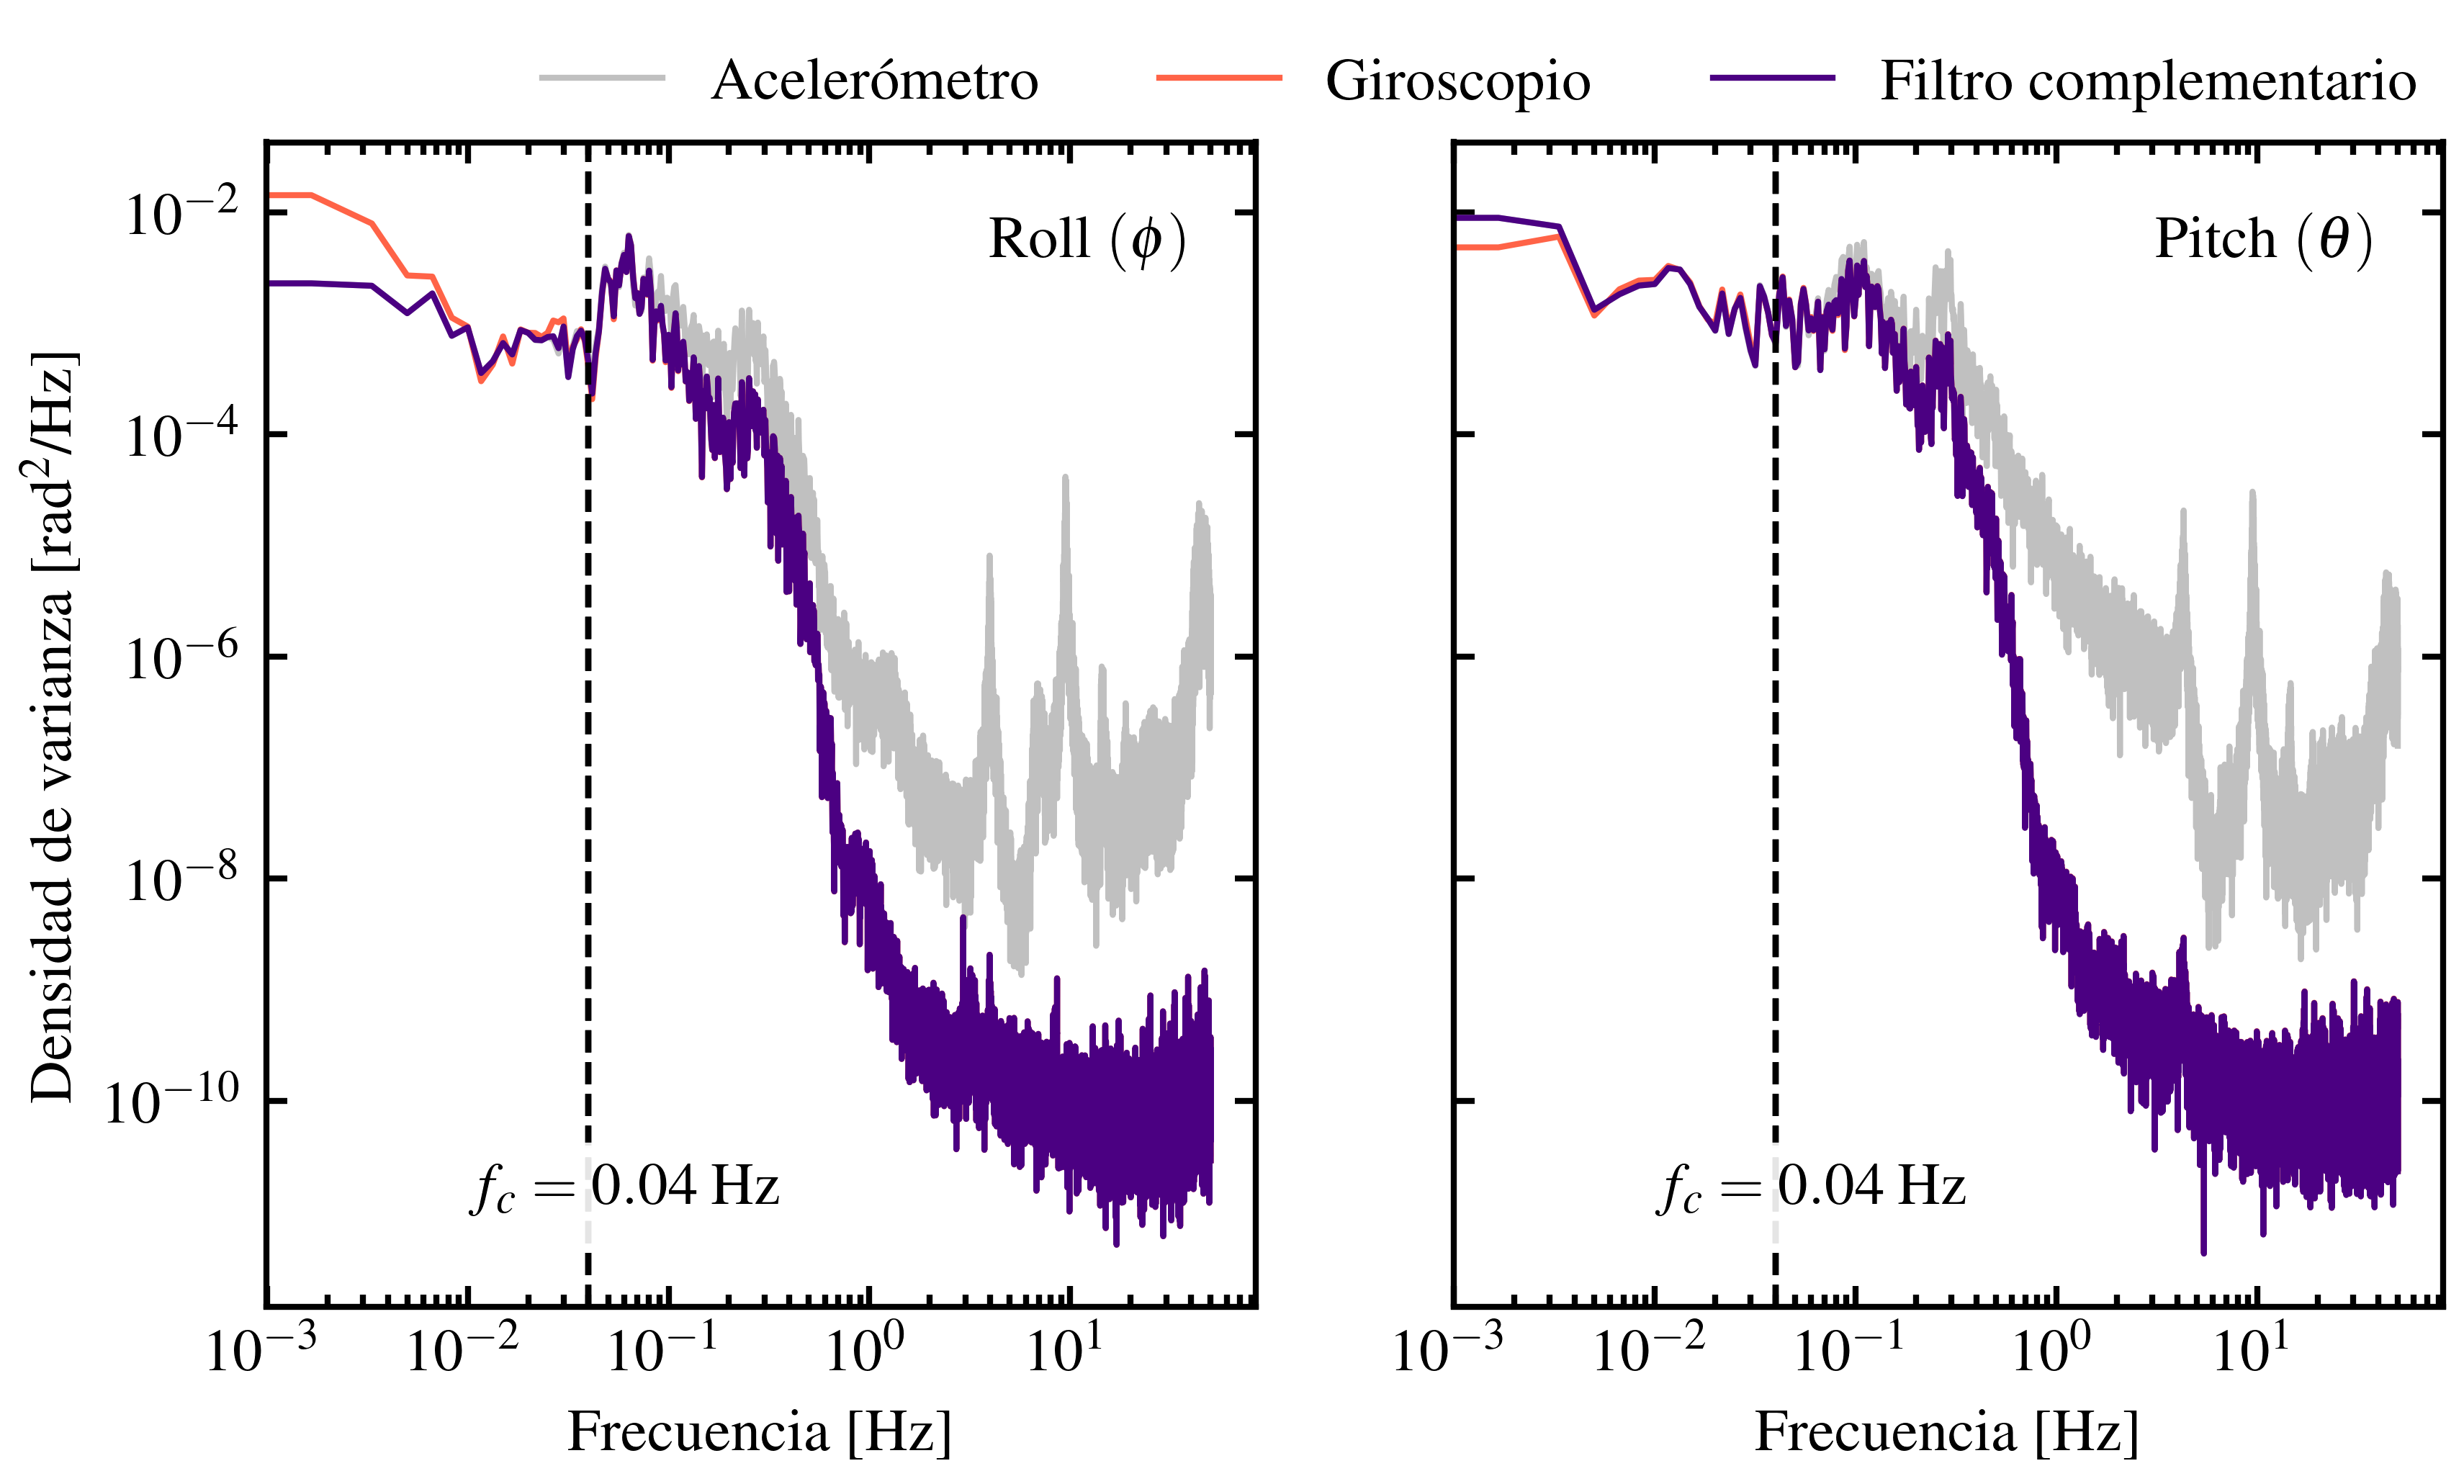
\includegraphics[width=0.87\linewidth]{./figures/spectra_pitch_and_roll.png}
  \caption{
    Espectro de densidad de varianza de las señales del angulo roll (izquierda)
    y pitch (derecha). Se compara el espectro de los datos obtenidos con el
    giroscopio (naranja), del acelerómetro (gris) y del filtro complementario
    (azul).
  }
  \label{fig:spectra_pitch_and_roll}
\end{figure}

% }}}

% Orientación de la boya {{{
\subsection{Cálculo de la orientación de la boya}

El otro ángulo que se tiene para completar los ángulos de Euler, es la
orientación de la boya. Este ángulo es especial, porque necesita que se defina
un punto de referencia, que generalmente es el norte. El acelerómetro es inútil
para calcular el ángulo de orientación, por lo que se requiere un magnetómetro o
brújula. La BOMM cuenta con dos instrumentos que tienen este tipo de sensor. Uno
de ellos es la estación meteorológica Gill Maximet GMX-600 y el otro es el AD2CP
Nortek Signature 1000 kHz. El Signature automáticamente entrega el valor del
``heading'' (orientación) con respecto al norte magnético, el cual es medido
como un ángulo en sentido horario entre 0 y 360. En el caso de la Maximet la
orientación se debe inferir a partir de la dirección del viento. Este
instrumento corrige la dirección del viento relativa a su marca de orientación,
sumándole un ángulo para obtener la dirección del viento respecto al norte
magnético, o dirección del viento corregida. Aprovechando esto, la orientación
se puede calcular usando la siguiente fórmula:

\begin{equation}
  \psi = \theta^{w}_\mathrm{true} - \theta^{w}_\mathrm{rel} - \Delta_\psi
\end{equation}

donde $\theta^w$ representa la dirección del viento y $\Delta_\psi$ es el ángulo
que forma la marca de la Maximet, con el norte de la boya.  Este ángulo fue
cercano a los $-60^\circ$ y a los $-180^\circ$ para las BOMM1-ITS y BOMM2-ITS,
respectivamente.  Por lo tanto, $\psi$ tiene un valor entre 0 y 360, y
representa la orientación del eje $x$ de la boya respecto al norte magnético y
es positivo en sentido horario.

\begin{figure}[htpb]
  \centering
  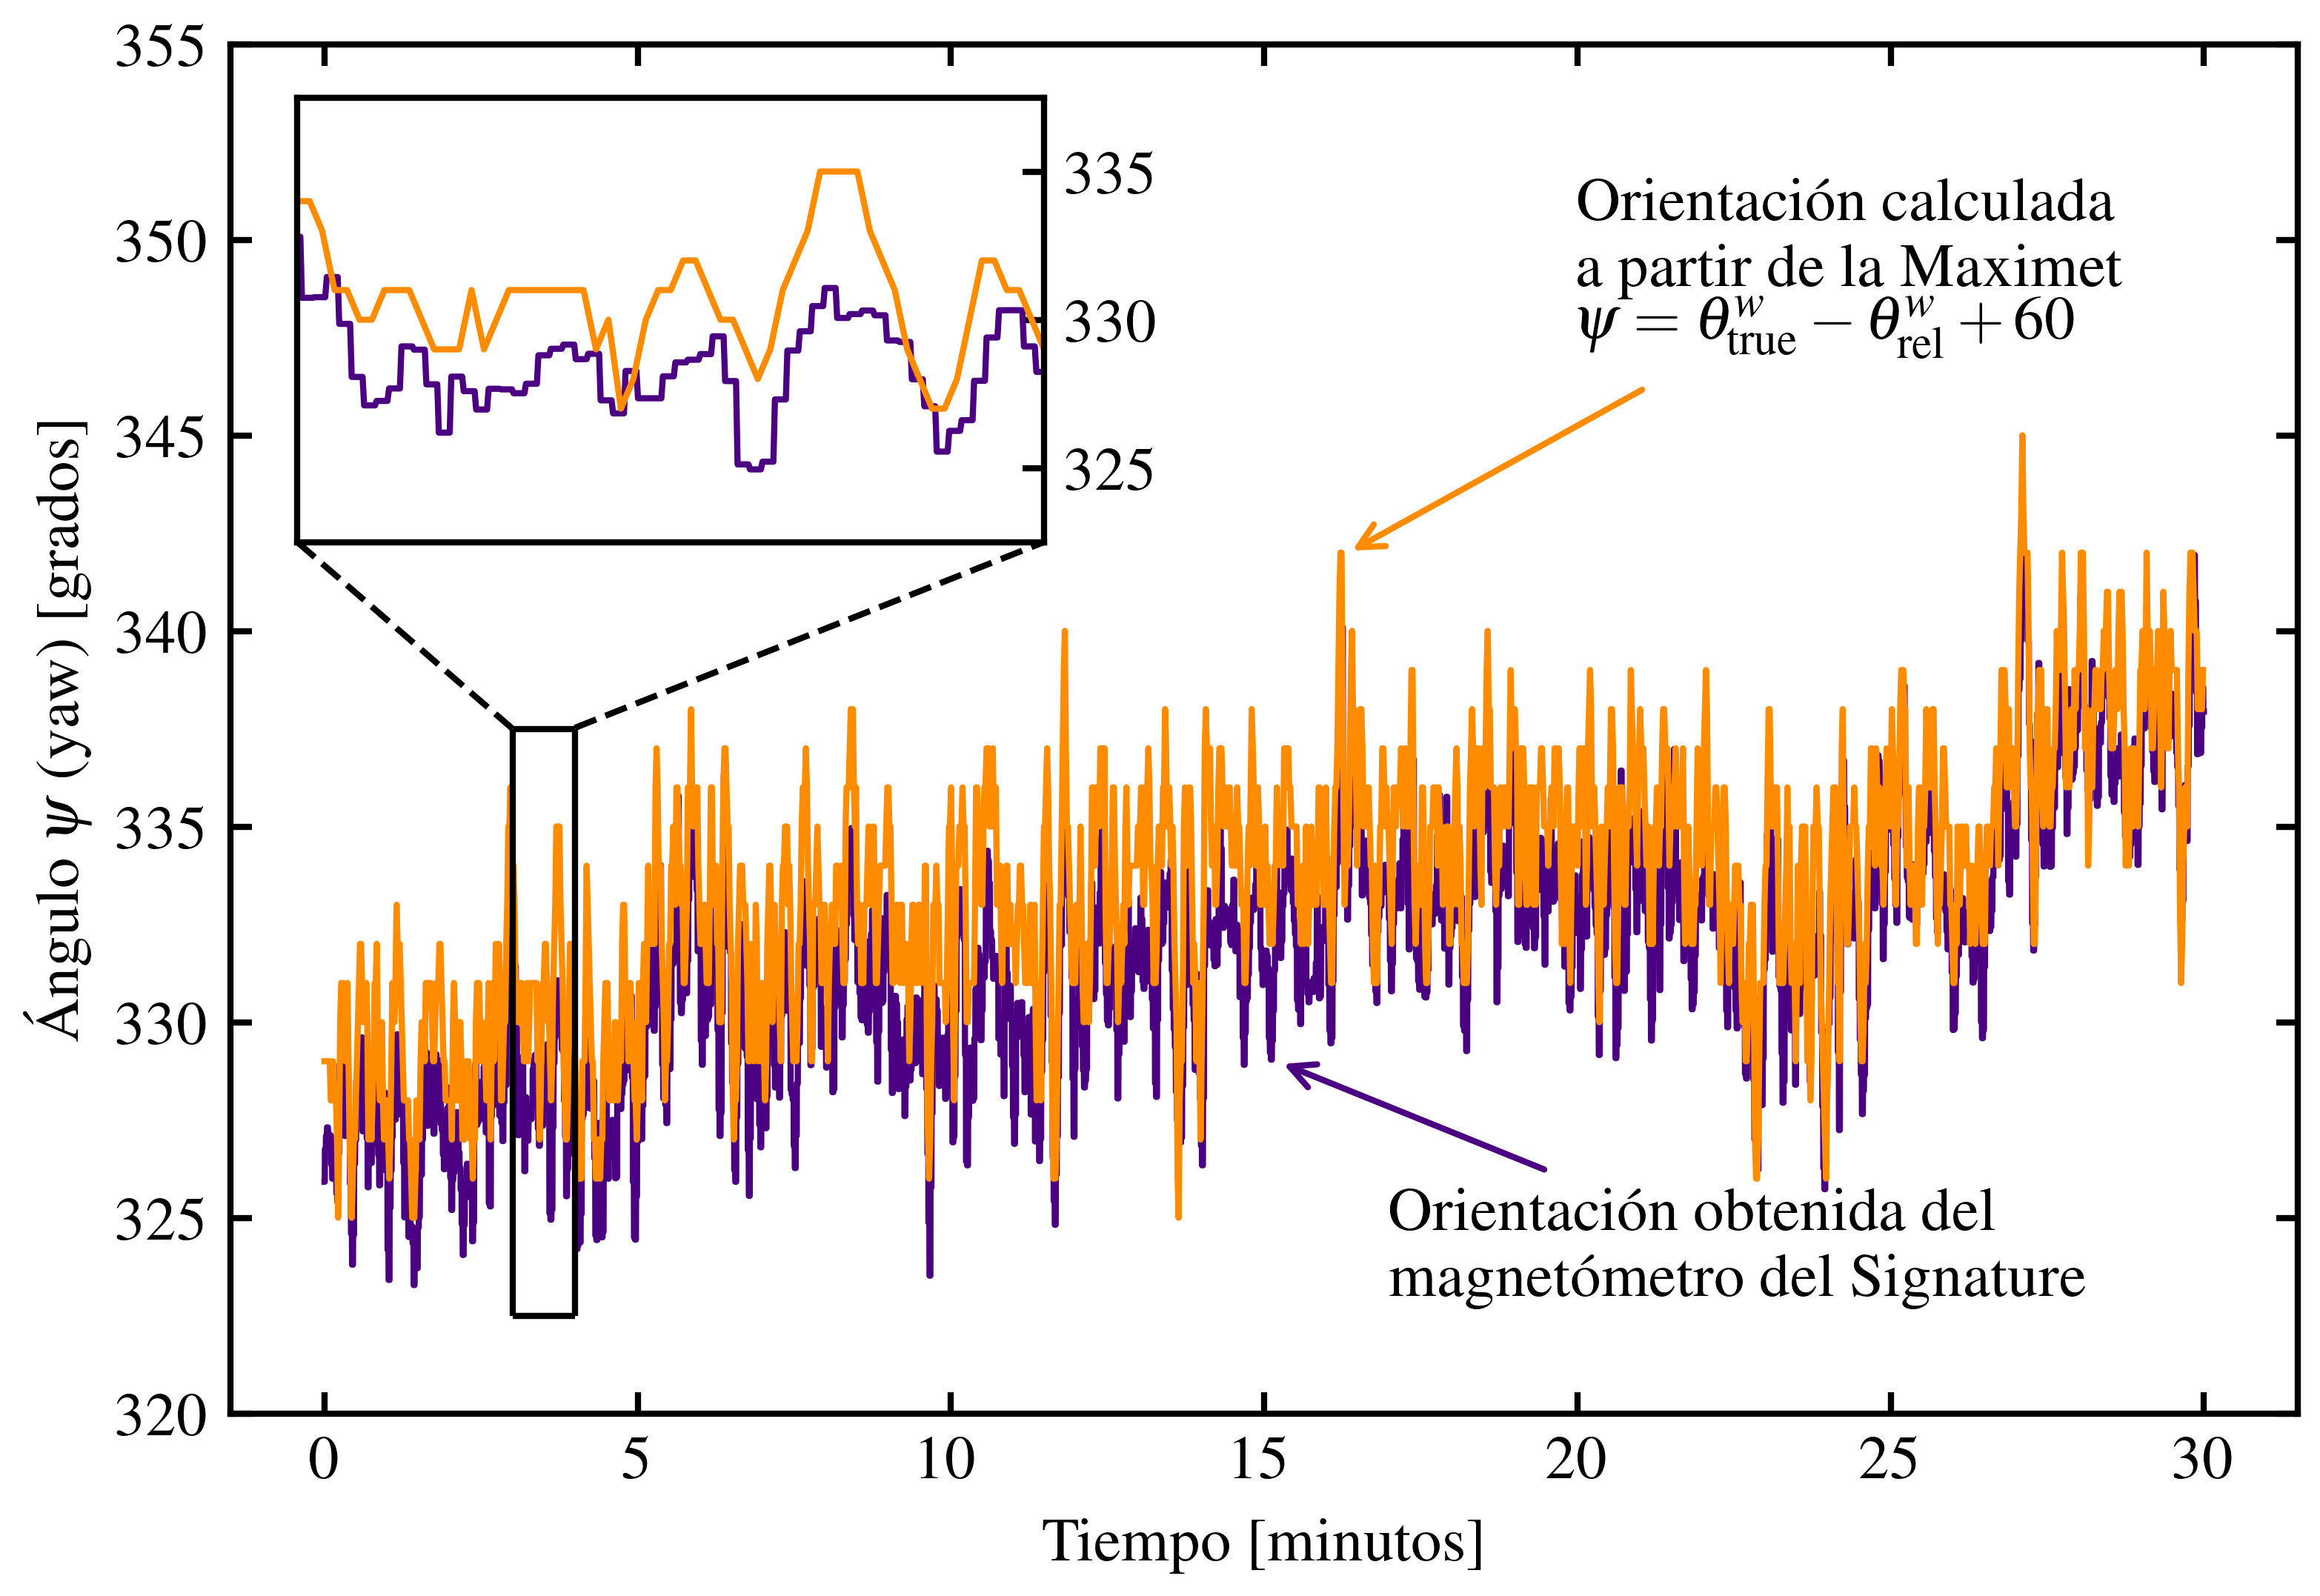
\includegraphics[width=0.8\linewidth]{./figures/heading_angle.png}
  \caption{Ángulo de orientación de la boya respecto al norte magnético.}
  \label{fig:heaging_angle}
\end{figure}

En la Fig.~\ref{fig:heaging_angle} se observa la comparación entre la
orientación obtenida del Signature y la estimada a partir de los datos de la
Maximet. Se podría decir que de forma general ambas señales se parecen bastante.
A pasar de esto, los datos del Signature se ven como cuadriculados y esto se
debe a que el valor del ``heading'' solo se actualiza cada segundo, pero el
instrumento arroja datos a 8 Hz. Por otro lado, se observa un sesgo entre los
datos de la Maximet y los datos del Signature, esto se debe posiblemente a un
error en la orientación de la Maximet. La recomendación es que siempre que se
pueda se usen los datos del Signature. Finlamente, el último paso es combinar
las señales de baja frecuencia (es decir las del magnetómetro, sea de la Maximet
o del Signature), con la señal de alta frecuencia calculada a partir de la
integración de la velocidad angular del giroscopio, de la misma manera que se
explicó en la sección anterior. Para ser más explícitos, la orientación final se
calcula como:

\begin{equation}
  \psi_{i} = \alpha \left[\psi_{i-1} + \dot{\psi_{i}} \Delta t \right] +
  (1-\alpha) \psi^\mathrm{mag}_{i}.
\end{equation}

Recordando que el punto de referencia es el norte magnético, un último paso es
sumarle al ángulo $\psi$ la declinación magnética, la cual se obtiene del GPS.
En el caso de Isla Todos Santos, la declinación magnética es de $11.2^\circ$.

% }}}

% Movimientos de la boya {{{
\subsection{Movimientos lineales de la boya}

Nos referimos a los movimientos lineales de la boya como las traslaciones que
se presentan en las tres direcciones, es decir, la traslación hacia adelante y
atrás (surge), la traslación lateral (sway) y la traslación vertical (heave). En
este caso se deben integrar las aceleraciones que son registradas por el IMU,
una vez para obtener la velocidad y dos veces para obtener la posición.
Al igual que al integrar los datos del giroscopio para obtener una estimación la
de la inclinación de la boya, se presenta una acumulación del error cuando se
integran los datos del acelerómetro, y esto se hace mucho más evidente cuando se
integra por segunda vez para obtener la posición.

Hay varias alternativas para solucionar este problema, la más sencilla es
aprovechar las propiedades de la transformada de Fourier y se hace una
integración en el dominio de la frecuencia, removiendo el ruido en las bajas
frecuencias. La transformada de Fourier de una serie de tiempo $x(t)$ se podría
definir como:

\begin{equation}
  \mathcal{F}\{x(t)\} = X(\omega) = \int x(t) e^{-i\omega t} \mathrm{d}t,
\end{equation}

por lo tanto, la doble integral es,

\begin{equation}
  \iint x(t)\mathrm{d}t = \mathcal{F}^{-1} \{(-i\omega)^{-2} X(\omega) \}.
\end{equation}

La ventaja de la integración en el dominio de la frecuencia es que se pueden
filtrar las oscilaciones de baja frecuencia. En este caso se aplicó la integral
para frecuencias mayores de $0.04\,\mathrm{Hz}$, es decir, descartando los
movimientos con períodos mayores que $25$ segundos. También se probó algunos
filtros ``pasa-bajas'' con frecuencias de corte en $4\,\mathrm{Hz}$ y en
$1\,\mathrm{Hz}$. En las Fig.~\ref{fig:motion_spectra} se muestra el espectro en
frecuencia del movimiento vertical registrado por el IMU comparado con el
espectro de la elevación de la superficie libre de uno de los alambres de
capacitancia. Se observa como cuando no se aplica un filtro que remueva la
energía en las bajas frecuencias, esta crece exponencialmente debido a la
``deriva.''

\begin{figure}[htpb]
  \centering
  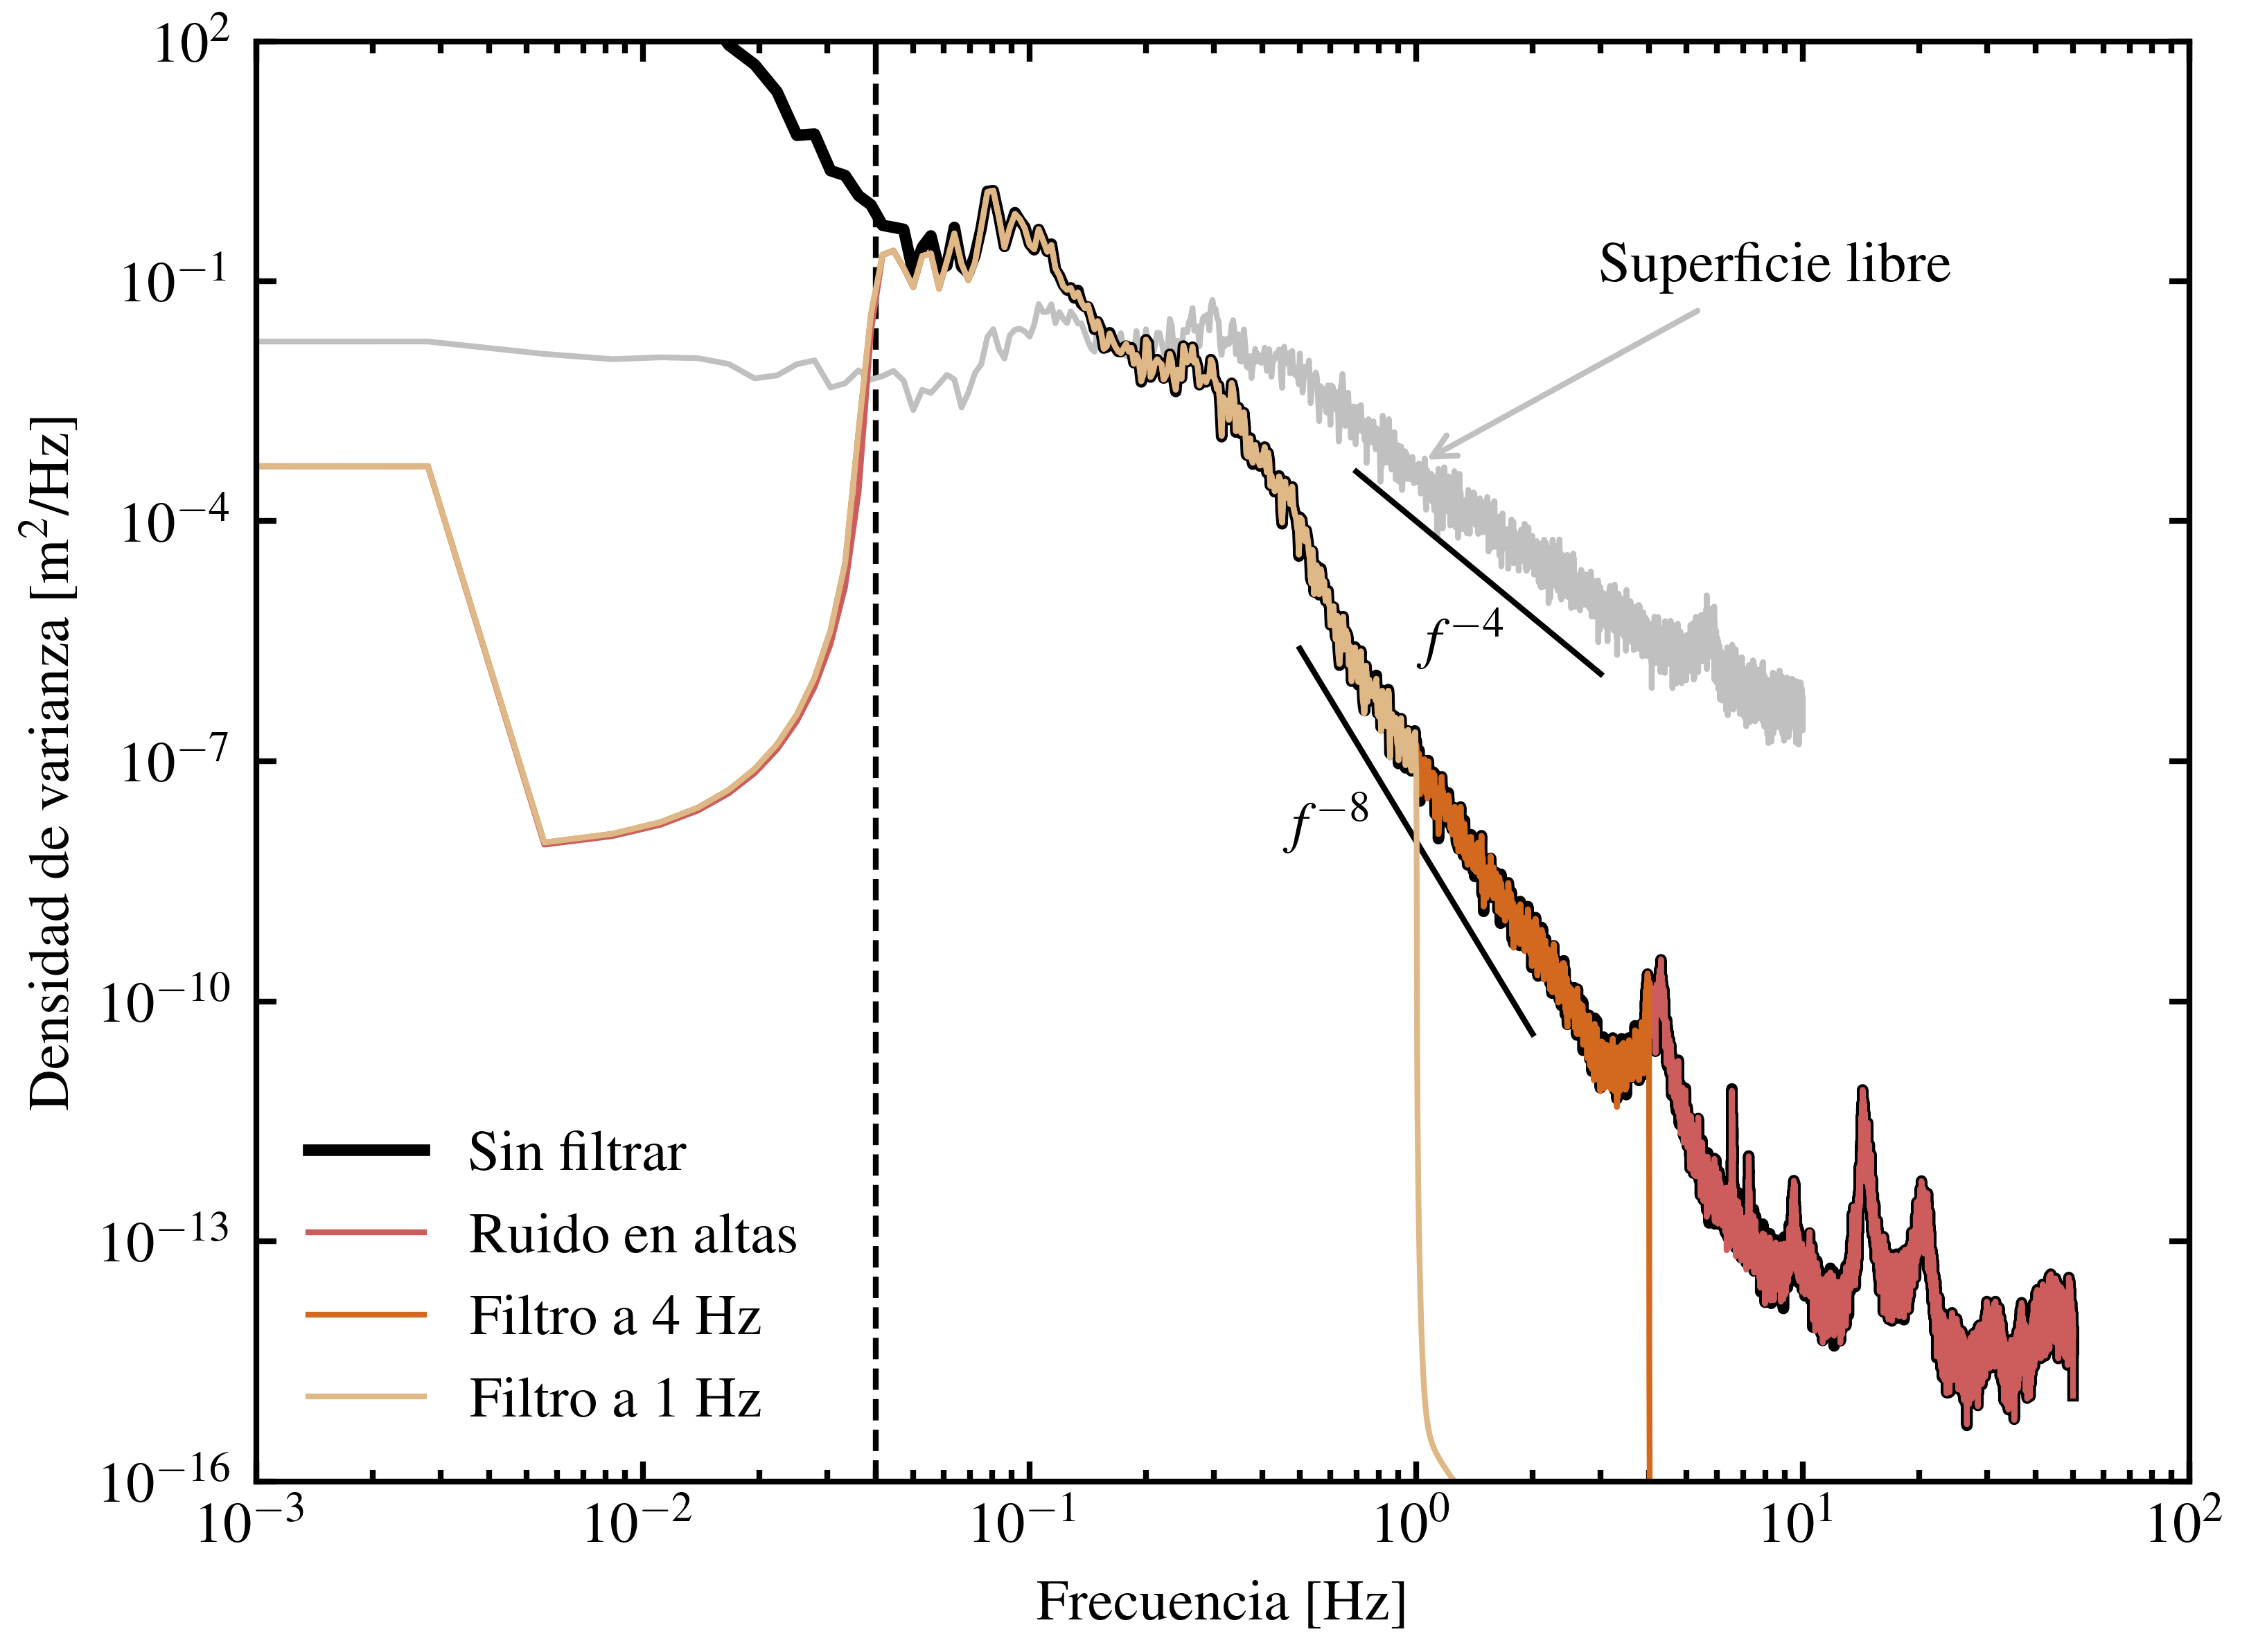
\includegraphics[width=0.8\linewidth]{./figures/motion_spectra.png}
  \caption{
    Espectro en frecuencia del movimiento lineal vertical del IMU comparados con
    la elevación de la superficie libre de uno de los alambres de capacitancia.
  }
  \label{fig:motion_spectra}
\end{figure}

% }}}

% }}}

% corrección de los datos {{{
\section{Corrección de los datos}

Las observaciones de la elevación de la superficie libre deben ser corregidas
para tener en cuenta el movimiento de la boya, es decir, se espera que la boya
se mueva con las olas más largas y las olas de más alta frecuencia que
atraviesan la boya queden registradas por el arreglo de a alambres de
capacitancia. Otra cosa a tener en cuenta es que la boya tiene a inclinarse
ligeramente lo que modifica la lectura de los alambres. Para corregir esto se
usa la siguiente ecuación:

\begin{equation}
  \mathbf{x}_\mathrm{E} =
    \mathbf{R} \mathbf{x}_\mathrm{B} + 
    \mathbf{R} \displaystyle\iint \mathbf{a}_\mathrm{B} \mathrm{d}t \mathrm{d}t +
    \mathbf{R} \int \boldsymbol{\Omega}_\mathrm{B} \times \mathbf{R} 
                \mathbf{L}_\mathrm{B} \mathrm{d}t.
\label{eq:surface_elevacion_correction}
\end{equation}

El término del lado izquierdo de la ecuación
\eqref{eq:surface_elevacion_correction} es el vector de elevación de la
superficie libre en el marco de referencia en tierra. El primer término del lado
derecho es la transformación del vector observado $\mathbf{x}_\mathrm{B}$ usando
la matriz de la ecuación \eqref{eq:rotation_matrix}. El segundo y el tercer
término representan la corrección debido a las traslaciones lineales y a la
inclinación de la boya, respectivamente. En la
Fig.~\ref{fig:surface_elevation_spectra} se presenta un ejemplo de los espectros
en frecuencia de los datos de elevación de la superficie libre y cada uno de los
términos que contribuye a la corrección, así mismo se presenta el espectro de
los datos corregidos. Se observa el mayor efecto de la corrección de los datos
de superficie libre en las bandas de frecuencias características del swell
(entre $0.05\;\mathrm{Hz}$ y $0.1\;\mathrm{Hz}$, lo que equivale a olas entre 10
y 20 segundos, respectivamente).

\begin{figure}[htpb]
  \centering
  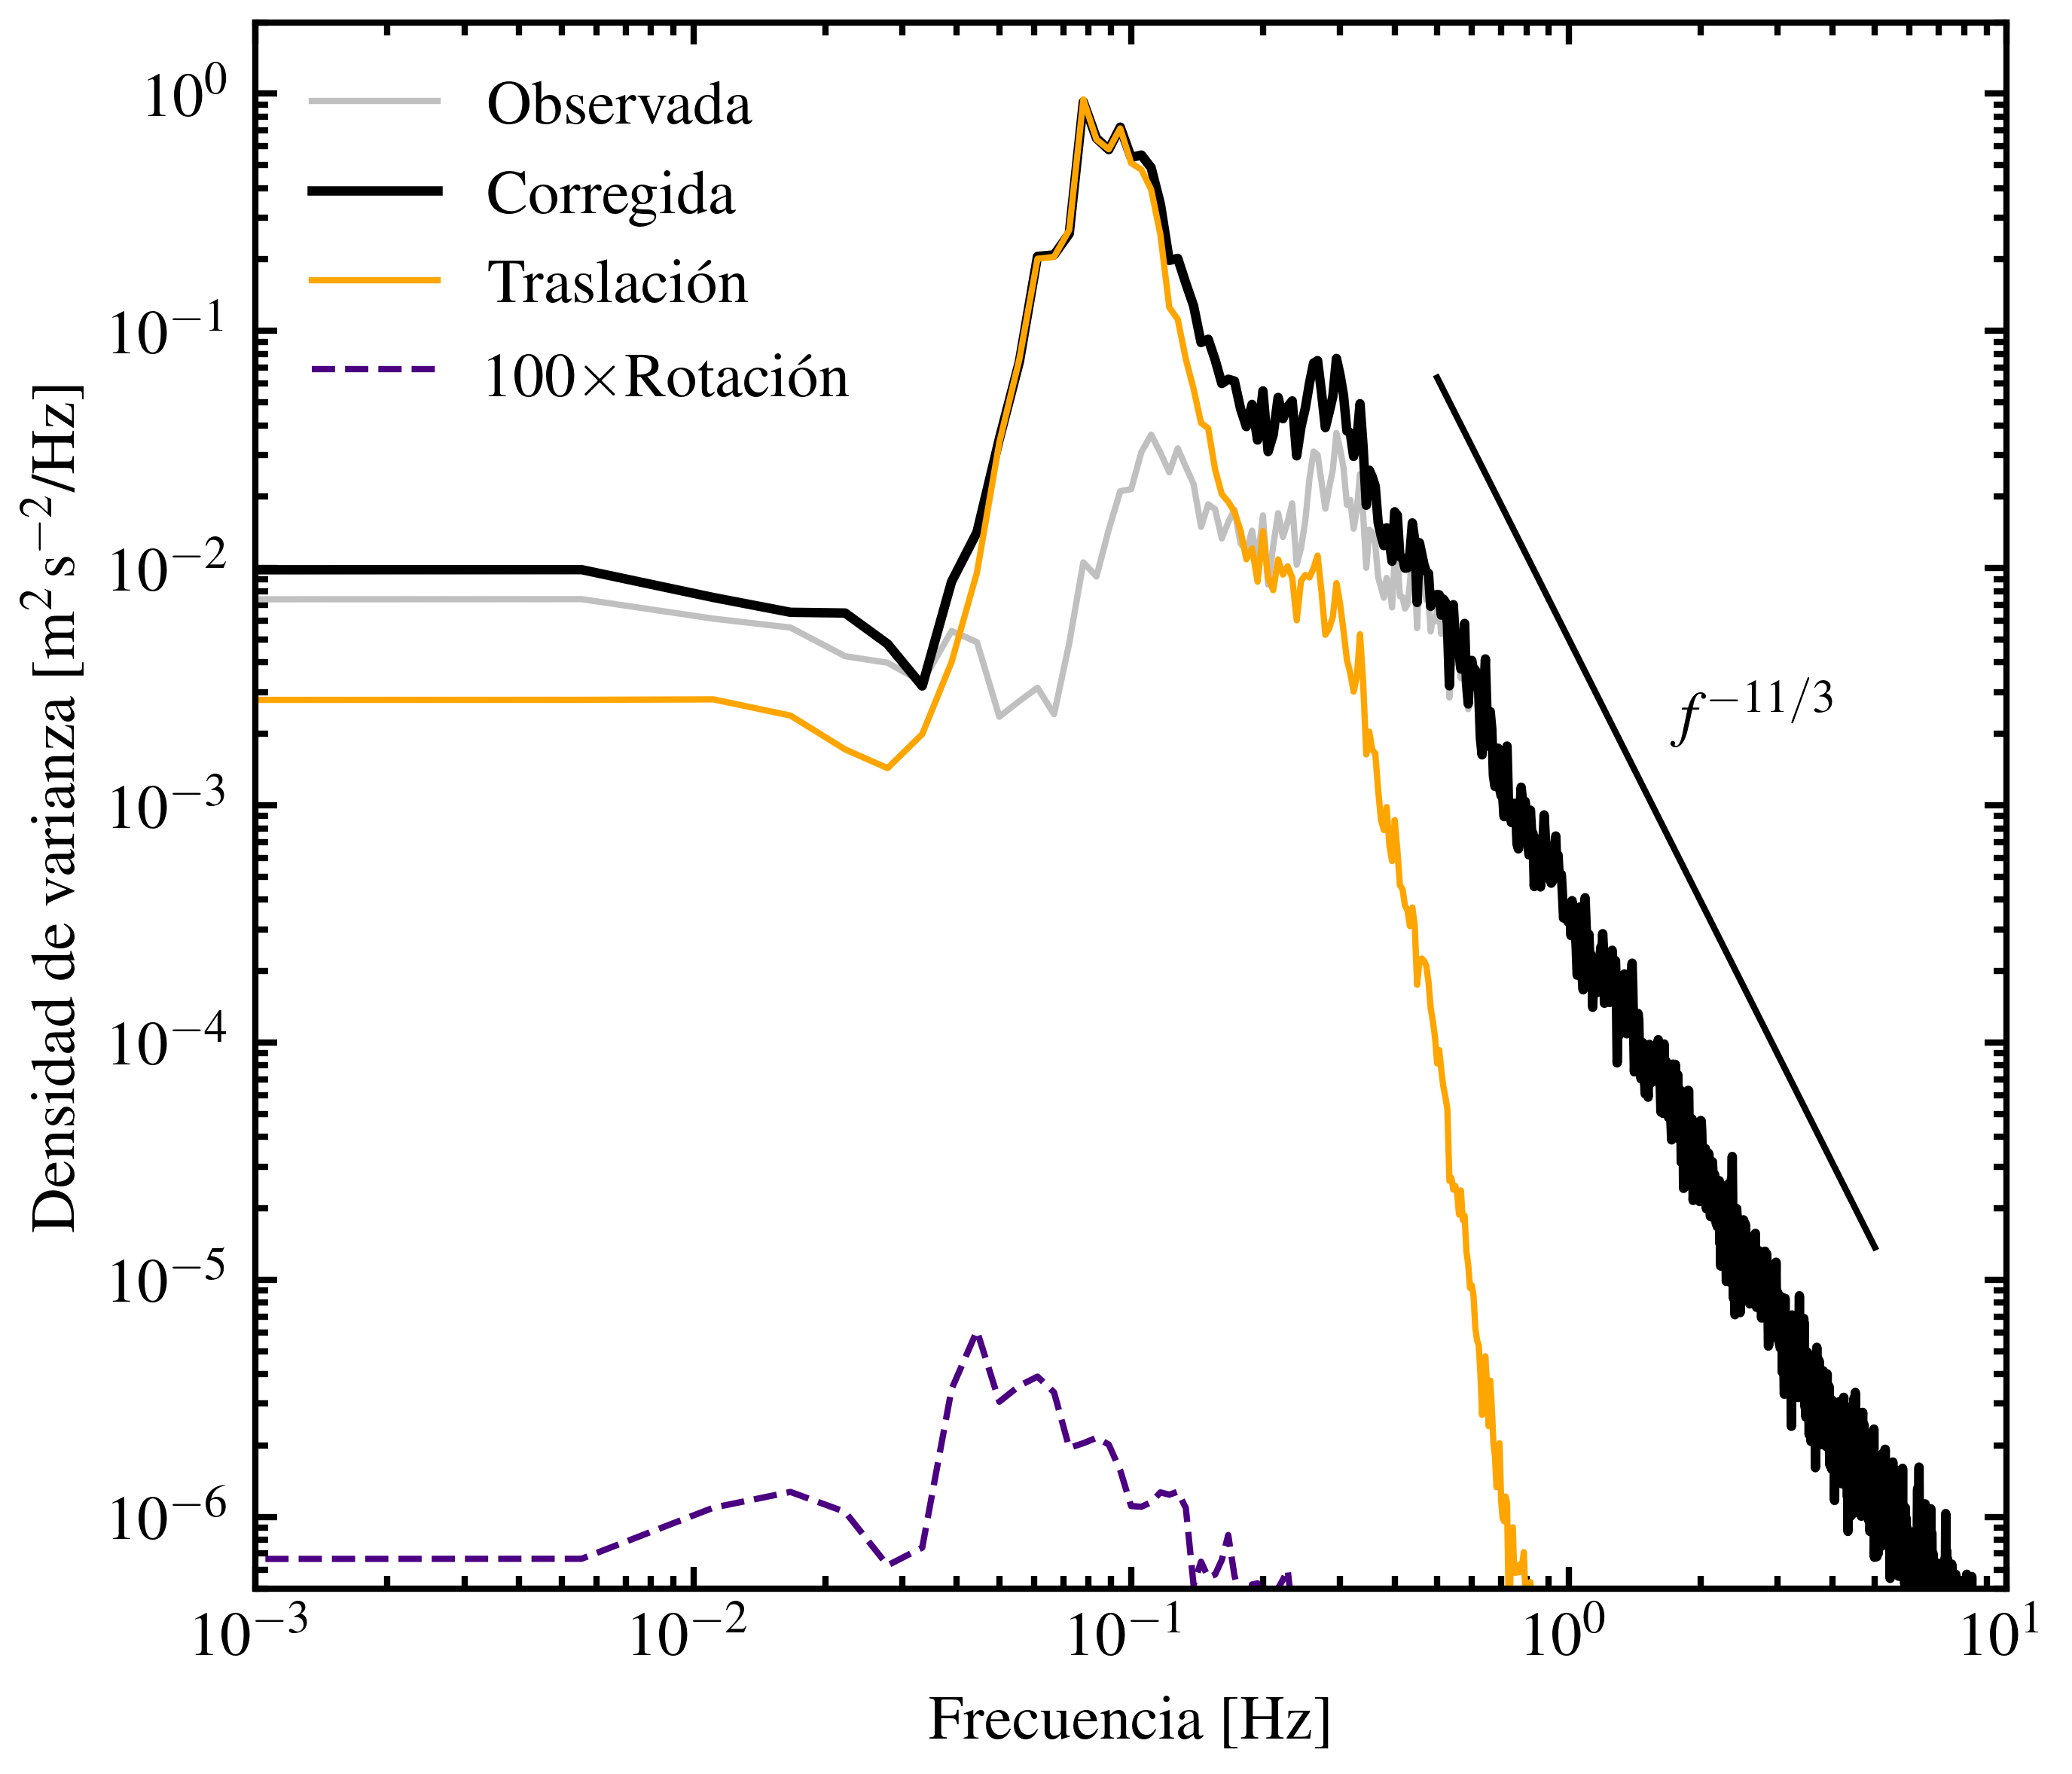
\includegraphics[width=0.7\linewidth]{./figures/surface_elevation_spectra.png}
  \caption{
    Efecto de la corrección de los datos de superficie libre debido al movimiento
    de la boya. Se muestran los espectros en frecuencia de cada una de las
    componentes de la ecuación \eqref{eq:surface_elevacion_correction}.
  }
  \label{fig:surface_elevation_spectra}
\end{figure}

La corrección que se hace al vector de velocidad del viento que se mide con el
anemómetro sónico funciona de la misma manera. En la ecuación
\eqref{eq:velocity_correction} se presentan los términos correspondientes,
análogos a la ecuación \eqref{eq:surface_elevacion_correction}, pero en este
caso las aceleraciones solo se integran una vez, para obtener la velocidad de
traslación de la boya.

\begin{equation}
  \mathbf{u}_\mathrm{E} =
    \mathbf{R} \mathbf{u}_\mathrm{B} + 
    \mathbf{R} \displaystyle\int
      \mathbf{a}_\mathrm{B} \mathrm{d}t +
      \mathbf{R} \left( \boldsymbol{\Omega}_\mathrm{B} \times
      \mathbf{L}_\mathrm{B} \right).
\label{eq:velocity_correction}
\end{equation}

En la Fig.~\ref{fig:velocity_spectra} se observa la contribución de cada uno de
los términos. Es importante notar que a diferencia de la superficie libre, los
datos de velocidad son altamente sensibles a la rotación de la boya, sin
embargo, la contribución más importante a la corrección de los datos, tanto de
velocidad del viento, como de elevación de la superficie libre, es la
translación lineal de la boya. 

\begin{figure}[htpb]
  \centering
  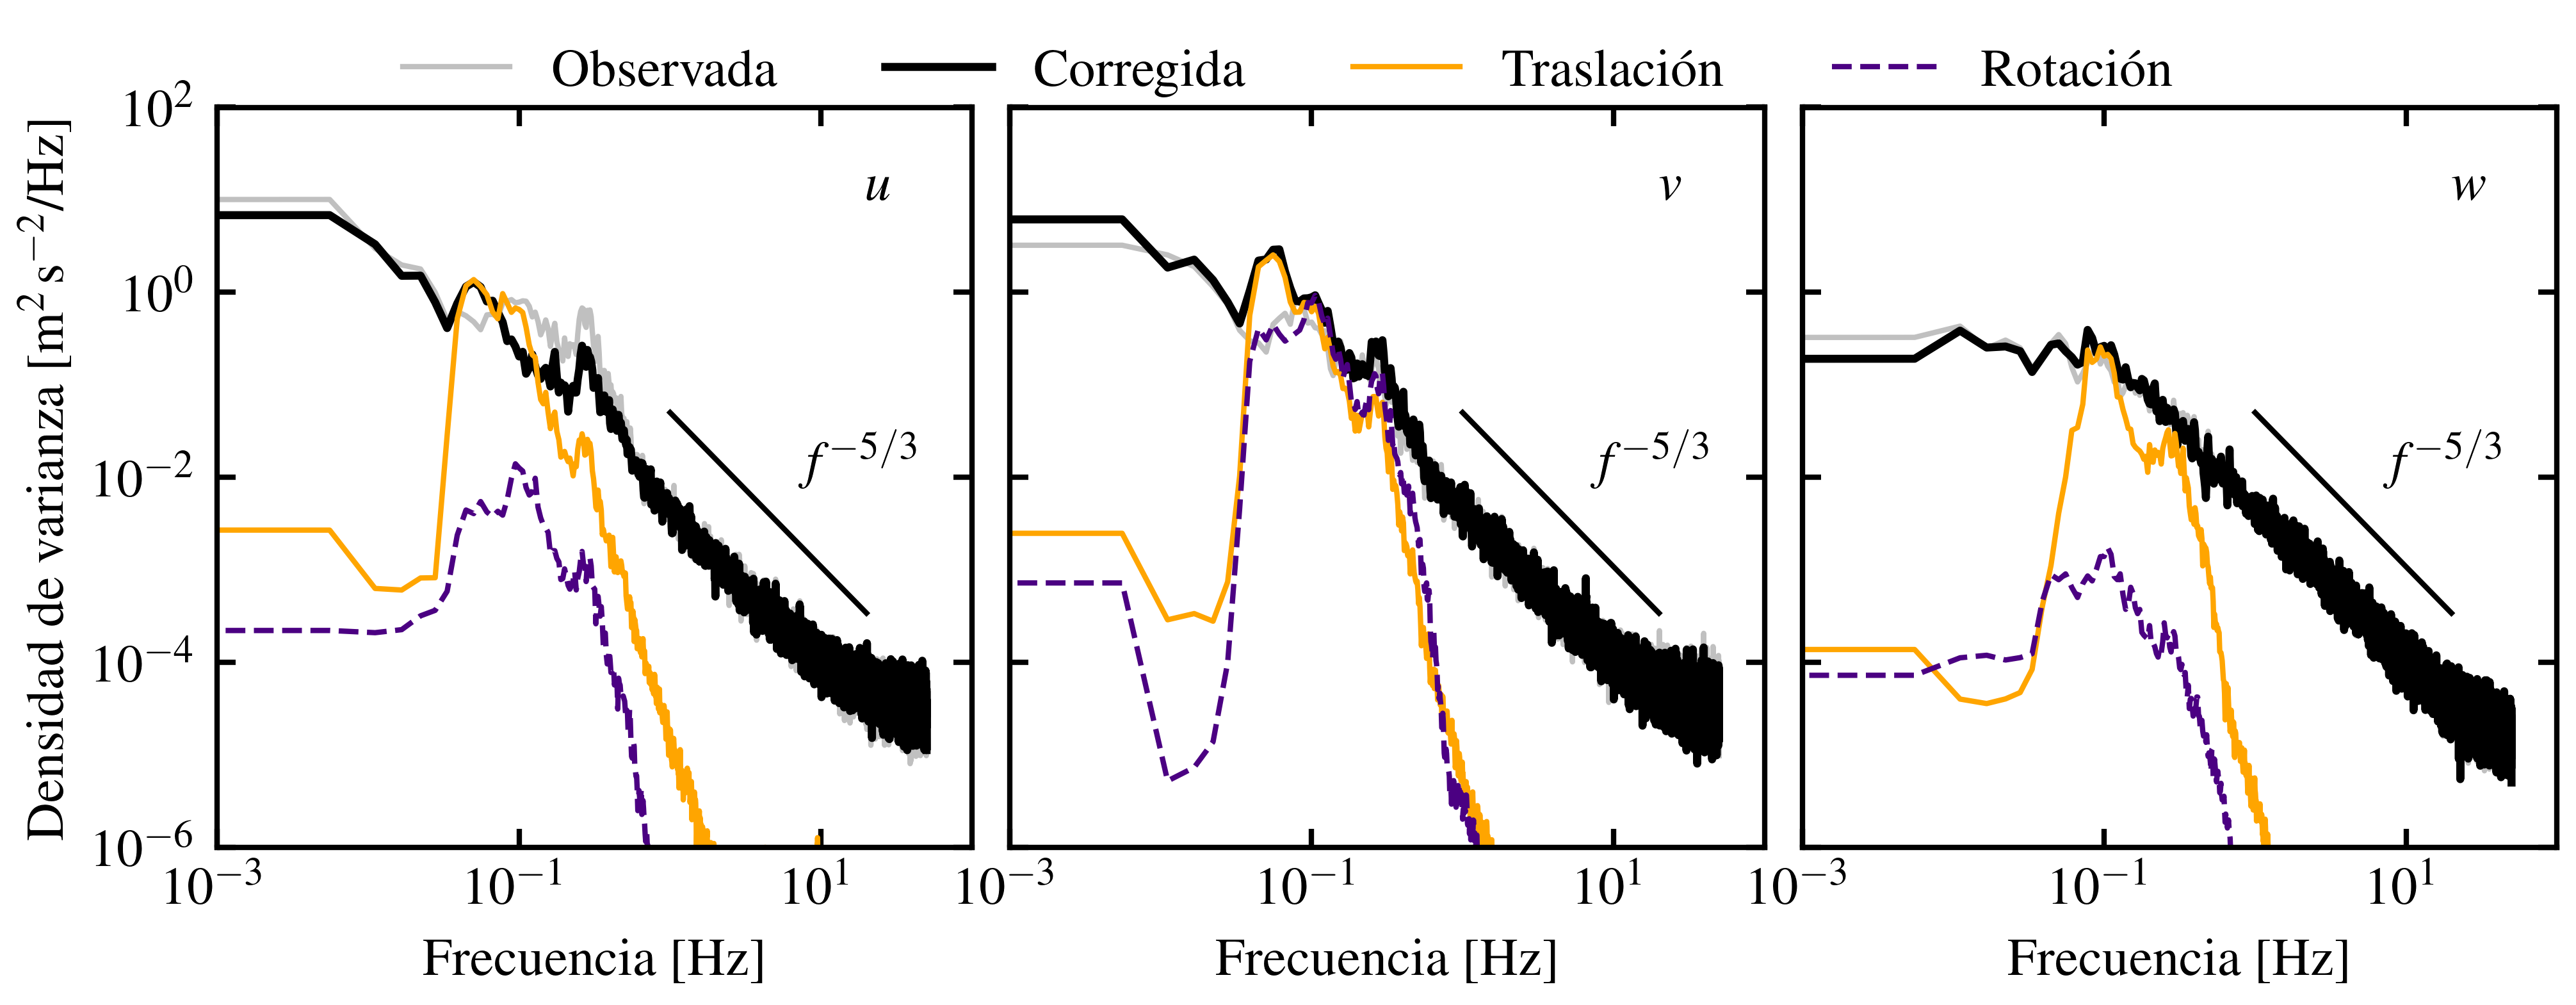
\includegraphics[width=\linewidth]{./figures/velocity_spectra.png}
  \caption{
    Espectro en frecuencia de las componentes $u$, $v$ y $w$ (paneles izquierdo,
    central y derecho respectivamente) de la velocidad del viento, antes y
    después de aplicar la corrección por el movimiento. Se muestran también cada
    una de las componentes de la ecuación \eqref{eq:velocity_correction} al
    igual que en la Fig.~\ref{fig:surface_elevation_spectra}.
  }
  \label{fig:velocity_spectra}
\end{figure}


\subsubsection*{Nota importante}%
\label{ssub:nota_importante}

Vale la pena mencionar que una de las variables más importantes
en el momento de aplicar la corrección de los datos por el movimientos de la
boya, es la posición relativa entre el IMU y el anemómetro sónico o el alambre
de capacitancia, en ambos casos denotado por $\mathbf{L}_\mathrm{B}$. Cada
componente de este vector, que está en el marco de referencia de la boya (por
lo tanto el subíndice $\mathrm{B}$), debe ser medido o estimado para cada una de
las boyas. Es importante notar que el sensor IMU no está alineado con el eje
central de la boya, si no que se encuentra excéntrico a este. En el caso de los
alambres de capacitancia la posición horizontal de cada alambre se estima
transformando las coordenadas polares (radio y ángulo) a coordenadas
cartesianas ($x$ y $y$, mientras que la coordenada vertical de cada alambre está
dada por la lectura que hace de la superficie libre más la altura del cero del
alambre respecto al IMU.


% }}}

%  finalizar documento --------------------------------------------------------
\end{document}
